% ===== 第一部分：单变量分析学 / 第8章：Riemann积分 =====
% !TEX root = ../../main.tex
\setchapterimage{figure/chapter8封面图.png}
\setchapterintro{这一章讲Riemann积分，囊括了不定积分,定积分与反常积分等内容，后面三章会分别讲这几个部分的一些命题和习题}
\chapter{Riemann积分}
% 第1节：不定积分
% !TEX root = ../../../main.tex
% 所属：第一部分：单变量分析学 / 第8章：Riemann积分
% 节：8.1 不定积分
% 正文按原文件顺序保存；由 ../chapter8.tex 调用。
\section{不定积分}
\begin{definition}
	设 \( y = f(x) \) ,在某个区间上,\( F'(x) = f(x) \),则称 \( F(x) \) 是 \( f(x) \) 的一个原函数或反导数,\( y = F(x) + \text{const} \) 是 \( y = f(x) \) 的原函数
	
\end{definition}
\begin{proposition}\label{原函数只差}
	在某区间上,若 \( f(x) \) 的任意两个原函数之差为常数.也即,设 \( F_1(x) \)、\( F_2(x) \) 为 \( f(x) \) 的原函数,则
	\[
	F_1(x) - F_2(x) = C
	\]
	
	
	
\end{proposition}
\begin{proof}
	\( F_1'(x) = F_2'(x) = f(x) \),在区间 \( I \) 上,令
	\[
	F(x) = F_1(x) - F_2(x)
	\]
	$
	F'(x) \equiv 0, \forall x \in I, \text{由 Rolle 定理,} F(x) = \text{Const.}$
\end{proof}
\begin{definition}
	在某区间上, \( f(x) \) 的不定积分定义为其所有原函数构成的集合,记作
	\[
	\int f(x) \dd x := \{ F(x) : F'(x) = f(x), \, x \in I \}
	\]
	
	由\ref{原函数只差} 等价于
	\[
	\int f(x) \dd x = \{ F(x) + C : \text{任意} F'(x) = f(x) \}
	\]
	
	为便于起见,记做
	\[
	\int f(x) \dd x = F(x) + C\]
	
\end{definition}
微分算子$\dd$与不定积分算子$\int$是一对逆运算,也就是说
$$\dd(\int f(x)\dd x)=f(x)\dd x\text{即}\dfrac{\dd}{\dd x}(\int f(x)\dd x)=f(x)$$
与$$\int\dd F(x)=F(x)+C$$成立

利用导数的性质,我们可以得到相应的积分的性质

利用导数的线性性质,有
\begin{proposition}
	在某区间$I$上, \( f(x) \),\( g(x) \) 的原函数都存在,则 \(\forall \, k_1, k_2 \in \mathbb{R}\),函数 \(k_1 f(x) + k_2 g(x)\) 的原函数也存在,且有
	\[
	\int [k_1 f(x) + k_2 g(x)] \dd x = k_1 \int f(x) \dd x + k_2 \int g(x) \dd x
	\]
	
\end{proposition}
注：等式两边都是函数族.
\begin{proof}
	设 \( F(x) \) 和 \( G(x) \) 分别是 \( f(x) \) 和 \( g(x) \) 的原函数,应有
	\[
	(k_1 F(x) + k_2 G(x))' = k_1 f(x) + k_2 g(x)
	\]
	
	那么
	\[
	\int (k_1 f(x) + k_2 g(x)) \dd x = k_1 F(x) + k_2 G(x) + C
	\]
	
	且
	\[\begin{aligned}
		k_1 \int f(x) \dd x + k_2 \int g(x) \dd x &= k_1 (F(x) + C_1) + k_2 (G(x) + C_2)\\	&= k_1 F(x) + k_2 G(x) + (k_1 C_1 + k_2 C_2)
	\end{aligned}\]
	
	
	上两式揭示的积分族相同,故
	\[
	\int [k_1 f(x) + k_2 g(x)] \dd x = k_1 \int f(x) \dd x + k_2 \int g(x) \dd x\]
\end{proof}
根据导数的乘法公式我们得到不定积分的分部积分公式
\begin{proposition}
	在某区间上,若有两个可微函数 $u(x), v(x)$,则
	\[
	\int u(x) v'(x) \dd x = u(x) v(x) - \int v(x) u'(x) \dd x
	\]
	经常简写为$$\int u \dd v = uv - \int v \dd u$$
	
\end{proposition}
\begin{proof}
	对 $u, v$ 有
	\[
	\dd(uv) = u \dd v + v \dd u
	\]
	
	两边积分,并移项得
	\[
	\int u \dd v = uv - \int v \dd u
	\]
	
	因此
	\[
	\int u(x) v'(x) \dd x = u(x) v(x) - \int v(x) u'(x) \dd x
	\]
\end{proof}

使用复合函数求导公式,我们得到第一类换元积分法.
\begin{proposition}
	对 $f(x)$,换元 $z = g(x)$,使 $f(x) = \tilde{f}(z )g'(x) = \tilde{f}(g(x)) \cdot g'(x)$.
	
	那么
	\[
	\int f(x) \dd x = \int \tilde{f}(g(x)) g'(x) \dd x = \int \tilde{f}(g(x)) \dd[g(x)] = \tilde{F}(g(x)) + C
	\]
	
	其中,$\tilde{F}(x)$ 为 $\tilde{f}(x)$ 的一个原函数.
\end{proposition}
类似的,有第二类换元积分法
\begin{proposition}
	对 $f(x)$,换元 $x = \varphi(t)$,其中 $\varphi(t)$ 是严格单调且可导,即其逆函数 $\varphi^{-1}$ 存在且可导
	\[\begin{aligned}
		\int f(x) \dd x &= \int f(\varphi(t)) \dd\varphi(t) = \int f(\varphi(t)) \cdot \varphi'(t) \dd t\\
		&= F(t) + C = F(\varphi^{-1}(x)) + C
	\end{aligned}\]
	
\end{proposition}\newpage
利用我们已经有的导数表,我们得到以下常用的积分公式
\begin{proposition}
	初等不定积分表：
	\[\begin{aligned}
		&(1)\int 0 \dd x = C\\
		&(2) \int x^\alpha \dd x = \frac{x^{\alpha+1}}{\alpha+1} + C \quad (\alpha \neq -1)\\
		&(3)\int \sin x \dd x = -\cos x + C\\
		&(4)\int \cos x \dd x = \sin x + C\\
		&(5)\int \sec^2 x \dd x = \tan x + C\\
		&(6)\int \csc^2 x \dd x = -\cot x + C\\
		&(7)\int \tan x \sec x \dd x = \sec x + C\\
		&(8)\int \cot x \csc x \dd x = -\csc x + C\\
		&(9)\int \frac{\dd x}{1-x^2} = \sin^{-1} x + C = -\cos^{-1} x + C\\
		&(10)\int \frac{\dd x}{1+x^2} = \tan^{-1} x + C = -\cot^{-1} x + C\\
		& (11) \int a^x \dd x = \frac{a^x}{\ln a} + C \quad (a > 0, a \neq 1)\\
		&(12) \int e^x \dd x = e^x + C\\
		&(13)\int \frac{1}{x} \dd x = \ln |x| + C\\
		&(14)\int \frac{1}{x \ln a} \dd x = \log_a |x| + C\\
		&(15)\int \sinh x \dd x = \cosh x + C\\
		&(16)\int \cosh x \dd x = \sinh x + C\\
		&(17)\int \text{sech}^2 x \dd x = \tanh x + C\\
		&(18)\int \frac{\dd x}{\sqrt{1+x^2}} = \sinh^{-1} x + C\\
		&(19)\int \frac{\dd x}{\sqrt{x^2-1}} = \cosh^{-1} x + C\\
		&(20)\int \frac{\dd x}{1-x^2} = \tanh^{-1} x + C
	\end{aligned}\]
\end{proposition}
此外还有一条相当好用的公式
\begin{proposition}
	\[\int\dfrac{f'(x)}{f(x)}\dd x=\ln|x|+C\]
\end{proposition}
这是第一类换元积分法的直接应用
%
% 第2节：一些例子,一些应用以及有理函数的积分
% !TEX root = ../../../main.tex
% 所属：第一部分：单变量分析学 / 第8章：Riemann积分
% 节：8.2 一些例子,一些应用以及有理函数的积分
% 正文按原文件顺序保存；由 ../chapter8.tex 调用。
\section{一些例子,一些应用以及有理函数的积分}
\begin{problem}
	计算以下不定积分：
	
	(1) $$\int \sin^2 x \dd x$$
	
	(2)$$\int \frac{(x+\sqrt{x})(x-2\sqrt{x})^2}{\sqrt{x}} \dd x$$
	
	(3) $$\int \frac{x^4}{1+x^2} \dd x$$
\end{problem}
\begin{solution}
	(1) 由于 $\sin^2 x = \dfrac{1}{2}(1 - \cos 2x)$,所以
	\[
	\int \sin^2 x \dd x = \frac{1}{2} \int (1 - \cos 2x) \dd x = \frac{1}{2} x - \frac{1}{2} \int \cos 2x \dd x
	\]
	\[
	= \frac{1}{2} x - \frac{1}{4} \sin 2x + C
	\]
	
	(2) \[\begin{aligned}
		\text{原式} &= \int \dfrac{x^3 - 2x^{5/2} + 4x^{3/2}}{x^{1/2}} \dd x\\& = \int (x^{5/2} - 3x^2 + 4x) \dd x\\
		&= \frac{2}{7} x^{7/2} -  x^3 + 2 x^3 + C
	\end{aligned}\]
	
	
	(3)\[\text{原式}= \int \frac{x^4 + x^2 - x^2}{1 + x^2} \dd x = \int \left(x^2 - 1 + \frac{1}{1+x^2}\right) \dd x= \frac{1}{3} x^3 - x + \tan^{-1} x + C\]  
\end{solution}
\begin{problem}
	(1)\[\int x\cos x\dd x\]
	(2)\[\int x^2e^x\dd x\]
	(3)\[\int\ln x\dd x\]
	(4)\[\int e^x\sin x\dd x\]
\end{problem}
\begin{solution}
	(1) $$\int x \cos x \dd x = \int x \dd\sin x = x \sin x - \int \sin x \dd x = x \sin x + \cos x + C$$
	
	(2)\[\begin{aligned}
		\int x^2 e^x \dd x &= \int x^2 \dd e^x = x^2 e^x - 2 \int x e^x \dd x\\&= x^2 e^x - 2 \int x \dd e^x = x^2 e^x - 2(x e^x - \int e^x \dd x) \\&= x^2 e^x - 2x e^x + 2 e^x + C = (x^2 - 2x + 2)e^x + C
	\end{aligned}\] 
	
	(3) $$\int \ln x \dd x = x \ln x - \int x \dd\ln x = x \ln x - \int x \cdot \frac{1}{x} \dd x = x \ln x - x + C$$
	
	(4) 设 $I = \displaystyle\int e^x \sin x \dd x$,$J = \displaystyle\int e^x \cos x \dd x$,
	\[
	\begin{cases}
		I = \displaystyle\int \sin x \dd e^x = e^x \sin x - \displaystyle\int e^x \cos x \dd x = e^x \sin x - J \\
		J = \displaystyle\int \cos x \dd e^x = e^x \cos x + \displaystyle\int e^x \sin x \dd x = e^x \cos x + I
	\end{cases}
	\]
	解得：
	\[
	I = \frac{1}{2} e^x (\sin x - \cos x) + C, \quad J = \frac{1}{2} e^x (\cos x + \sin x) + C
	\]
\end{solution}
\begin{problem}
	(1)$$\int\frac{\dd x}{x^2+a^2}\text{与}\int \frac{\dd x}{\sqrt{a^2-x^2}}$$
	(2)$$\int\tan x\dd x\text{与}\int\cot x\dd x$$
	(3)$$\int\sec x\dd x\text{与}\int\csc x\dd x$$
	(4)$$\int\frac{\dd x}{\sqrt{x}(1+x)}$$
\end{problem}
\begin{solution}
	(1)
	\[
	\int \frac{\dd x}{x^2 + a^2} = \frac{1}{a} \int \frac{\dd\left(\dfrac{x}{a}\right)}{\left(\dfrac{x}{a}\right)^2 + 1} = \frac{1}{a} \tan^{-1} \frac{x}{a} + C
	\]
	
	\[
	\int \frac{\dd x}{\sqrt{a^2-x^2}} = \int \frac{\dd\left(\dfrac{x}{a}\right)}{1 - \sqrt{\left(\dfrac{x}{a}\right)^2}} = \sin^{-1} \dfrac{x}{a} + C
	\]
	
	(2)
	\[
	\int \tan x \dd x = \int \frac{\sin x}{\cos x} \dd x = -\ln |\cos x| + C
	\]
	
	\[
	\int \cot x \dd x = \int \frac{\cos x}{\sin x} \dd x = \ln |\sin x| + C
	\]
	
	(3)
	\[
	\int \sec x \dd x = \int \frac{\sec x (\sec x + \tan x)}{\sec x + \tan x} \dd x = \ln |\sec x + \tan x| + C
	\]
	
	\[
	\int \csc x \dd x = \int \frac{\csc x (\csc x - \cot x)}{\csc x - \cot x} \dd x = -\ln |\csc x - \cot x| + C
	\]
	
	(4)
	\[
	\int \frac{\dd x}{x \sqrt{1 + x}} = 2 \int \frac{\dd(\sqrt{x})}{1 + (\sqrt{x})^2} = 2 \tan^{-1} \sqrt{x} + C
	\]
\end{solution}
\begin{problem}
	(1)\[\int \sqrt{a^2-x^2}\dd x\]
	(2)\[\int\frac{\dd x}{\sqrt{x^2-a^2}}\text{和}\int\frac{\dd x}{\sqrt{x^2+a^2}}\]
	(3)\[\int \sqrt{x^2+a^2}\dd x\text{和}\int \sqrt{x^2-a^2}\dd x\]
\end{problem}
\begin{solution}
	(1) 设 $x = a \sin \theta$,则 $\dd x = a \cos \theta \dd \theta$,
	\[\begin{aligned}
		\int \sqrt{a^2 - x^2} \dd x &= \int a^2 \cos^2 \theta \dd \theta = a^2 \int \frac{1 + \cos 2\theta}{2} \dd \theta\\
		&= \frac{1}{2} a^2 \theta + \frac{1}{4} a^2 \sin 2\theta + C\\	&= \frac{1}{2} a^2 \sin^{-1} \frac{x}{a} + \frac{1}{2} a^2 \cdot \frac{x}{a^2} \sqrt{a^2 - x^2} + C\\&= \frac{1}{2} x \sqrt{a^2 - x^2} + \frac{a^2}{2} \sin^{-1} \frac{x}{a} + C
	\end{aligned}\]
	(2) 设 $x = a \sec \theta$,则 $\dd x = a \sec \theta \tan \theta \dd \theta$,
	\[\begin{aligned}
		\int \frac{\dd x}{ \sqrt{x^2 - a^2}} &= \int \frac{a \sec \theta \tan \theta \dd \theta}{ a \tan \theta} = \int \sec \theta \dd \theta = \ln |\sec \theta + \tan \theta| + C\\&= \ln \left| \frac{x}{a} + \frac{\sqrt{x^2 - a^2}}{a} \right| + C = \ln \left| x + \sqrt{x^2 - a^2} \right| + C
	\end{aligned}\]
	
	
	同理
	\[
	\int \frac{\dd x}{\sqrt{x^2 + a^2}} = \ln \left| x + \sqrt{x^2 + a^2} \right| + C
	\]
	(3) 考虑 $\displaystyle\int \sqrt{x^2 + a^2} \dd x$：
	
	\[\begin{aligned}
		\int \sqrt{x^2 + a^2} \dd x &= x \sqrt{x^2 + a^2} - \int \frac{x^2}{\sqrt{x^2 + a^2}} \dd x\\& = x \sqrt{x^2 + a^2} + \int \frac{a^2}{\sqrt{x^2 + a^2}} \dd x - \int \sqrt{x^2 + a^2} \dd x
	\end{aligned}\]
	
	移项得：
	\[
	2 \int \sqrt{x^2 + a^2} \dd x = x \sqrt{x^2 + a^2} + a^2 \ln \left| x + \sqrt{x^2 + a^2} \right| + C
	\]
	
	因此：
	\[
	\int \sqrt{x^2 + a^2} \dd x = \frac{1}{2} \left( x \sqrt{x^2 + a^2} + a^2 \ln \left| x + \sqrt{x^2 + a^2} \right| \right) + C
	\]
	
	同理
	\[
	\int \sqrt{x^2 - a^2} \dd x = \frac{1}{2} \left( x \sqrt{x^2 - a^2} - a^2 \ln \left| x + \sqrt{x^2 - a^2} \right| \right) + C
	\]
\end{solution}
这样我们得到基本积分表的下半部分
\begin{proposition}
	(1) $$\int \tan x \dd x = -\ln |\cos x| + C$$
	
	(2) $$\int \cot x \dd x = \ln |\sin x| + C$$
	
	(3) $$\int \sec x \dd x = \ln |\sec x + \tan x| + C$$
	
	(4) $$\int \csc x \dd x = \ln |\csc x - \cot x| + C$$
	
	(5) $$\int \frac{\dd x}{\sqrt{x^2 \pm a^2}} = \ln \left| x + \sqrt{x^2 \pm a^2} \right| + C$$
	
	(6)$$\int \frac{\dd x}{\sqrt{a^2 - x^2}} =  \sin^{-1} \frac{x}{a} + C$$
	
	(7) $$\int \frac{\dd x}{x^2 - a^2} = \frac{1}{2a} \ln \left| \frac{x - a}{x + a} \right| + C$$
	
	(8) $$\int \frac{\dd x}{x^2 + a^2} = \frac{1}{a} \tan^{-1} \frac{x}{a} + C$$
	
	(9) $$\int \sqrt{a^2 - x^2} \dd x = \frac{1}{2} x \sqrt{a^2 - x^2} + \frac{a^2}{2} \sin^{-1} \frac{x}{a} + C$$
	
	(10)$$\int \sqrt{x^2 \pm a^2} \dd x = \frac{1}{2} \left( x \sqrt{x^2 \pm a^2} \pm a^2 \ln \left| x + \sqrt{x^2 \pm a^2} \right| \right) + C$$
\end{proposition}
\begin{problem}计算下列积分
	\begin{enumerate}
		\item[(1)]
		$\displaystyle \int \frac{\dd x}{\sqrt{x^2 + 2\xi x + \eta^2}}$
		
		\item[(2)]
		$\displaystyle \int \frac{ax + b}{\sqrt{x^2 + 2\xi x + \eta^2}} \dd x$
		
		\item[(3)]
		$\displaystyle \int \frac{ax + b}{x^2 + 2\xi x + \eta^2} \dd x$
		
		\item[(4)]
		$\displaystyle \int (ax + b) \sqrt{x^2 + 2\xi x + \eta^2} \dd x$
	\end{enumerate}
	
\end{problem}
\begin{solution}
	(1)\[\int \frac{\dd x}{\sqrt{x^2 + 2\xi x + \eta^2}} = \int \frac{\dd(x + \xi)}{\sqrt{(x + \xi)^2 \pm |\eta^2 - \xi^2|}} = \ln \left| x + \xi + \sqrt{x^2 + 2\xi x + \eta^2} \right| + C\]
	(2)$$\begin{aligned}
		&\int \frac{ax + b}{x^2 + 2\xi x + \eta^2} \dd x
		= \frac{a}{2} \int \frac{\dd(x^2 + 2\xi x + \eta^2)}{x^2 + 2\xi x + \eta^2} + (b - a\xi) \int \frac{\dd x}{(x+\xi)^2+\eta^2-\xi^2} \\
		&= \begin{cases}
			a \ln \left| x + \xi  \right| - \dfrac{b - a\xi}{x+\xi}  + C, & |\xi| =|\eta| \\
			\dfrac{a}{2} \ln \left| x^2 + 2\xi x + \eta^2 \right| + \dfrac{b - a\xi}{\sqrt{\eta^2 - \xi^2}} \arctan\dfrac{x+\xi}{\sqrt{\eta^2-\xi^2}} + C, & |\xi| < |\eta| \\
			\dfrac{a}{2} \ln \left| x^2 + 2\xi x + \eta^2 \right| + \dfrac{b - a\xi}{2\sqrt{\xi^2 - \eta^2}}\ln \left| \dfrac{x + \xi - \sqrt{\xi^2 - \eta^2}}{x + \xi + \sqrt{\xi^2 + \eta^2}} \right|  + C, & |\xi| > |\eta|
		\end{cases}
	\end{aligned}$$
	
	(3)\[\begin{aligned}
		\int \frac{ax + b}{\sqrt{x^2 + 2\xi x + \eta^2}} \dd x
		&= \dfrac{a}{2} \int \frac{\dd(x^2 + 2\xi x + \eta^2)}{\sqrt{x^2 + 2\xi x + \eta^2}} + (b - a\xi) \int \frac{\dd x}{\sqrt{x^2 + 2\xi x + \eta^2}} \\
		&= \sqrt{x^2 + 2\xi x + \eta^2} +(b - a\xi)\ln|x+\xi+ \sqrt{x^2 + 2\xi x + \eta^2}|+C
	\end{aligned}\]
	(4)\[\begin{aligned}
		&\int(ax+b) \sqrt{x^2 + 2\xi x + \eta^2}\dd x\\
		=&\dfrac{a}{2}\int \sqrt{x^2 + 2\xi x + \eta^2}\dd( x^2 + 2\xi x + \eta^2)+(b-a\xi)\int \sqrt{x^2 + 2\xi x + \eta^2}\dd x\\
		=&\dfrac{a}{3} (x^2 + 2\xi x + \eta^2)^{3/2}+\frac{b-a\xi}{2}[(x+\xi) \sqrt{x^2 + 2\xi x + \eta^2}+(\eta^2-\xi^2)\ln|x+\xi+ \sqrt{x^2 + 2\xi x + \eta^2}|]+C
	\end{aligned}\]
\end{solution}
\begin{problem}\label{积分10}
	(1)$$I_n=\int \frac{\dd x}{(x^2+a^2)^n}$$
	(2)\[I_n\int x^ne^x\dd x\]
	(3)\[I_n=\int\cos^nx\dd x\]
\end{problem}
\newpage
\begin{solution}
	(1)对于 $n \geq 2$：
	
	\begin{align*}
		I_n &= \int \frac{\dd x}{(x^2 + a^2)^n} \\
		&= \frac{1}{a^2} \int \frac{\dd x}{(x^2 + a^2)^{n-1}} - \frac{1}{a^2} \int \frac{x^2}{(x^2 + a^2)^n} \dd x \\
		&= \frac{I_{n-1}}{a^2} + \frac{1}{2a^2(n-1)} \int x \, d\left[ \frac{1}{(x^2 + a^2)^{n-1}} \right] \\
		&= \frac{I_{n-1}}{a^2} + \frac{1}{2a^2(n-1)} \left( \frac{x}{(x^2 + a^2)^{n-1}} - \int \frac{\dd x}{(x^2 + a^2)^{n-1}} \right) \\
		&= \frac{I_{n-1}}{a^2} + \frac{1}{2a^2(n-1)} \cdot \frac{x}{(x^2 + a^2)^{n-1}} - \frac{I_{n-1}}{2a^2(n-1)} \\
		&= \frac{2n-3}{2a^2(n-1)} I_{n-1} + \frac{1}{2a^2(n-1)} \cdot \frac{x}{(x^2 + a^2)^{n-1}}
	\end{align*}
	\[\begin{cases}
		I_n= \dfrac{2n-3}{2a^2(n-1)} I_{n-1} + \dfrac{1}{2a^2(n-1)} \cdot \dfrac{x}{(x^2 + a^2)^{n-1}}\\
		I_1=\dfrac{1}{a}\arctan\dfrac{x}{a}+C
	\end{cases}\]
	(2)\[
	I_n = \int x^n e^x \dd x = x^n e^x - \int e^x \dd(x^n) = x^n e^x - n \int x^{n-1} e^x \dd x = x^n e^x - n I_{n-1}
	\]
	
	所以,
	\[
	I_n + n I_{n-1} = x^n e^x
	\]
	
	有初值
	\[
	I_1 = \int x e^x \dd x = x e^x - \int e^x \dd x = (x - 1)e^x + C
	\]
	(3)\[\begin{aligned}
		I_n &= \int \cos^n x \dd x = \int \cos^{n-1} x \cdot \cos x \dd x = \int \cos^{n-1} x \dd(\sin x)\\&= \cos^{n-1} x \sin x + (n-1) \int \sin^2 x \cos^{n-2} x \dd x\\&= \cos^{n-1} x \sin x + (n-1) \int (1 - \cos^2 x) \cos^{n-2} x \dd x\\&	= \cos^{n-1} x \sin x + (n-1) I_{n-2} - (n-1) I_n
	\end{aligned}\]
	整理得：
	
	\[
	I_n = \frac{1}{n} \cos^{n-1} x \sin x + \left(1 - \frac{1}{n}\right) I_{n-2}
	\]
\end{solution}
\begin{problem}(有理函数的积分)
	给定 $P_m(x), Q_n(x) \in \mathbb{R}[x]$,且 $m = \deg P_m$,$n = \deg Q_n$,计算有理函数的积分：
	
	\[
	\int \frac{P_m(x)}{Q_n(x)} \dd x
	\]
\end{problem}
\begin{solution}
	若\( m \geqslant n \),由带余除法 
	
	\[
	P_m(x) = g(x) Q_n(x) + \tilde{P}_m(x)
	\]
	
	所以,
	
	\[
	\frac{P_m(x)}{Q_n(x)} = g(x) + \frac{\tilde{P}_m(x)}{Q_n(x)}, \quad \deg \tilde{P}_m < \deg Q_n
	\]
	
	其中 \( g(x) \) 是多项式,直接积分即可,后面只需考虑 \( n > m \) 的情况,由代数基本定理：
	
	\[
	Q_n(x) = (x - \alpha_1)^{m_1} \cdots (x - \alpha_t)^{m_t} (x^2 + 2\xi_1 x + \eta_1^2)^{n_1} \cdots (x^2 + 2\xi_s x + \eta_s^2)^{n_s}
	\]
	
	其中 \(\alpha_k, \xi_k, \eta_k \in \mathbb{R}\) 且 \(\xi_k^2 - \eta_k^2 < 0\)
	
	对 \(\dfrac{P_m(x)}{Q_n(x)}\) 写出部分分式分解的形式.
	
	每一个一次项：$(x - \alpha_k)^{m_k}$ 对应的展开形式：
	
	\[
	\frac{\lambda_{k1}}{x - \alpha_k} + \frac{\lambda_{k2}}{(x - \alpha_k)^2} + \cdots + \frac{\lambda_{km_k}}{(x - \alpha_k)^{m_k}}
	\]
	
	每一个二次项：$(x^2 + 2\xi_k x + \eta_k^2)^{n_k}$ 对应的展开形式：
	
	\[
	\frac{\mu_{k1}x + \nu_{k1}}{x^2 + 2\xi_k x + \eta_k^2} + \frac{\mu_{k2}x + \nu_{k2}}{(x^2 + 2\xi_k x + \eta_k^2)^2} + \cdots + \frac{\mu_{kn_k}x + \nu_{kn_k}}{(x^2 + 2\xi_k x + \eta_k^2)^{n_k}}
	\]
	
	这些系数可以由待定系数法得出
	
	只需考虑
	
	1.
	\[
	\int \frac{\dd x}{(x - \alpha)^n} =
	\begin{cases}
		\ln |x - \alpha| + C, & n = 1 \\
		\dfrac{1}{1-n} \cdot \dfrac{1}{(x - \alpha)^{n-1}} + C, & n >1
	\end{cases}
	\]
	
	2.\[\begin{aligned}
		\int \frac{\mu x + \nu}{(x^2 + 2\xi x + \eta^2)^n} \dd x &= \frac{\mu}{2} \int \frac{\dd(x^2 + 2\xi x + \eta^2)}{(x^2 + 2\xi x + \eta^2)^n} + (\nu-2\xi) \int \frac{\dd x}{(x^2 + 2\xi x + \eta^2)^n}\\&= \dfrac{\mu}{2(1-n)} \cdot \frac{1}{(x^2 + 2\xi x + \eta^2)^{n-1}} + (\nu-2\xi) I_n
	\end{aligned}\]
	$I_n=\displaystyle\int\dfrac{\dd x}{(x^2+2\xi x+\eta^2)^n}=\displaystyle\int\dfrac{\dd x}{((x+\xi)^2\pm|\eta^2-\xi^2|)^n}$,由\ref{积分10}得
\end{solution}
\begin{problem}
	(可化成有理函数的形式)
	令 \( R(u, v) \)表示关于两个变量 \( u, v \) 的有理函数（分母,分子为二元有理函数）,考虑以下类型的积分：
	
	1.
	\[
	\int R\left(x, \sqrt[n]{\frac{\xi x+\eta}{\mu x+\nu}}\right) \dd x
	\]
	
	2.
	\[
	\int R(\sin x, \cos x) \dd x
	\] 
	
\end{problem}
\begin{solution}
	
	1. 设
	\[
	t = \sqrt[n]{\frac{\xi x+\eta}{\mu x+\nu}}, x = \varphi(t) = \frac{-\nu t^n + \eta}{\mu t^n - \xi}
	\]
	
	则
	\[
	\int R\left(x, \sqrt[n]{\frac{\xi x+\eta}{\mu x+\nu}}\right) \dd x = \int R\left(\frac{-\nu t^n + \eta}{\mu t^n - \xi}, t\right) \varphi'(t) \dd t
	\]
	
	2. 令 \(\tan \dfrac{x}{2} = t\)
	\[
	\sin x = 2 \sin \frac{x}{2} \cos \frac{x}{2} = \frac{2t}{1 + t^2}, \cos x = \frac{1 - t^2}{1 + t^2},  \dd x = \dd(2 \arctan t) = \frac{2 \dd t}{1 + t^2}
	\]
	
	因此
	\[
	\int R(\sin x, \cos x) \dd x = \int R\left(\frac{2t}{1 + t^2}, \frac{1 - t^2}{1 + t^2}\right) \frac{2}{1 + t^2} \dd t
	\]
\end{solution}
\begin{problem}
	\[\int \frac{\dd x}{x(\sqrt[3]{x}-\sqrt{x})}\]
\end{problem}

\begin{solution}
	令$x=t^6,\dd x=6t^5\dd t$
	\[\int \frac{\dd x}{x(\sqrt[3]{x}-\sqrt{x})}=6\int \frac{\dd t}{t^3(1-t)}=6(\ln|\frac{\sqrt[6]{x}}{\sqrt[6]{x}-1}|-\frac{1}{\sqrt[6]{x}}-\frac{1}{2\sqrt[3]{x}})+C\]
\end{solution}

%
% 第3节：Riemann积分的定义以及可积性
% !TEX root = ../../../main.tex
% 所属：第一部分：单变量分析学 / 第8章：Riemann积分
% 节：8.3 Riemann积分的定义以及可积性
% 正文按原文件顺序保存；由 ../chapter8.tex 调用。
\section{Riemann积分的定义以及可积性}
\begin{definition}
	区间 \([a, b]\) 上的分划$P$定义为 一列点$x_0,x_1,\cdots,x_n\in[a,b]$,满足\[  a = x_0 < x_1 < x_2 < \cdots < x_n = b, x_k \in [a, b]\]
	定义分划 \(P\) 的模长为 \(\lambda = \max\limits_{1 \leq k \leq n} \Delta x_k\)
\end{definition}
\begin{definition}(常义积分)
	设 \( f(x) \) 在 \([a, b]\) 上有界,\(I\) 是一个常数,若对任意划分  
	\[
	P: a = x_0 < x_1 < \cdots < x_n = b
	\]  
	以及在 \([x_{k-1}, x_k]\) 任取的 \(\xi_k \in [x_{k-1}, x_k]\), \(k = 1, 2, \cdots, n\),当 \(\lambda(P) \to 0\) 时,Riemann 和  
	\[
	S = \sum_{k=1}^n f(\xi_k) \Delta x_k
	\]  
	有极限 \(I\),且不依赖于划分的方式和 \(\xi_1, \cdots, \xi_n\) 的选取,称 \(f(x)\) 在 \([a, b]\) 上 Riemann 可积或 Riemann 积分存在.  
	其积分值记为 \(I\),记为  
	\[
	I = \int_a^b f(x) \dd x.
	\]  
	
	\(b\) 为积分上限,\(a\) 为积分下限.\(f(x)\) 为被积函数.\(\dd x\) 中的 \(x\) 称为积分变量.
	
	这里的极限不是数列或者函数极限,用 \(\varepsilon\)-\(\delta\) 语言定义为：  
	$\forall \varepsilon > 0, \exists \delta > 0, $使得对任意划分  
	\[
	P: a = x_0 < x_1 < \cdots < x_n = b
	\]  
	与任意选取的 \(\xi_i \in [x_{i-1}, x_i]\),只要  
	\[
	\lambda = \max_{1 \leq i \leq n} (\Delta x_i) < \delta,
	\]  
	便有  
	\[
	\left| \sum_{i=1}^n f(\xi_i) \Delta x_i - I \right| < \varepsilon.
	\]  
	
	则称 \( f(x) \) 在 \([a, b]\) 上 Riemann 可积.记为 \( f \in \mathcal{R}[a, b] \).
\end{definition}
\begin{example}
	讨论 \( D(x) \) 在 \([0,1]\) 上的可积性
\end{example}
\begin{solution}
	\(\forall P: a = x_0 < x_1 < \cdots < x_n = b, \forall[x_{i-1}, x_i]  \exists a \in \mathbb{Q}, b \in \mathbb{Q}^c\),  
	满足 \(a \in [x_{i-1}, x_i], b \in [x_{i-1}, x_i]\).
	
	取 $\xi_i$ 为有理数
	
	\[\lim_{\lambda \to 0} \sum_{i=1}^n f(\xi_i) \Delta x_i = \lim_{\lambda \to 0} \sum_{i=1}^n 1 \cdot \Delta x_i = 1\]
	
	$\xi_i$ 为无理数
	
	\[\lim_{\lambda \to 0} \sum_{i=1}^n f(\xi_i) \Delta x_i = \lim_{\lambda \to 0} \sum_{i=1}^n 0 \cdot \Delta x_i = 0\]
	
	
\end{solution}
上面的定义方式依赖于$I$的选取,下面介绍另一种考察可积性的方式
\begin{definition}
	
	设 $f(x)$ 在 $[a,b]$ 上有界,对 $[a,b]$ 的一个划分
	\[
	P: a = x_0 < x_1 < \cdots < x_n = b
	\]
	在 $[x_{k-1}, x_k]$ 上
	\[
	M_k = \sup_{x \in [x_{k-1}, x_k]} f(x), \quad m_k = \inf_{x \in [x_{k-1}, x_k]} f(x)
	\]
	存在且唯一,称
	\[
	\overline{S}(P) = \sum_{k=1}^n M_k \Delta x_k
	\]
	为 Darboux 大和；
	\[
	\underline{S}(P) = \sum_{k=1}^n m_k \Delta x_k
	\]
	为 Darboux 小和.
	
\end{definition}


注意 Darboux 和不是 Riemann 和的特殊形式,例如
\[
f(x)=
\begin{cases}
	1-x, & x>0 \\[4pt]
	0, & x=0 \\[4pt]
	x-1, & x<0
\end{cases}
\]
在 $(-\varepsilon, \varepsilon)$ 上的 Darboux 和不可能是 Riemann 和.
\begin{definition}
	将一个分划的加细定义为在一个划分的分点上加入新的分点
\end{definition}
\begin{lemma}\label{大和不增,小和不减}
	设 $f(x)$ 在 $[a,b]$ 上有界,设 $P: x_0 = a < x_1 < \cdots < x_n = b$ 为 $[a,b]$ 的一个划分,对 $P$ 的加细后,大和不增,小和不减.
\end{lemma}
\begin{proof}
	仅需证明在 $P$ 中插入一个新分点后结果成立即可.现考虑大和,
	\[
	P': x_0 = a < x_1 < \cdots < x_{k-1} < x_k' < x_k < \cdots < x_n = b
	\]
	令
	\[
	M_k' = \sup_{x \in [x_{k-1}, x_k']} f(x), \quad M_k'' = \sup_{x \in [x_k', x_k]} f(x)
	\]
	\[
	\begin{aligned}
		\overline{S}(P') - \overline{S}(P) &= M_k'(x_k' - x_{k-1}) + M_k''(x_k - x_k') - M_k(x_k - x_{k-1}) \\
		&\leq M_k(x_k' - x_{k-1}) + M_k(x_k - x_k') - M_k(x_k - x_{k-1}) = 0
	\end{aligned}
	\]
	
	对小和同理.
\end{proof}
\begin{lemma}
	$f(x)$ 在 $[a,b]$ 上有界,设
	\[
	P': a = x_0' < x_1' < \cdots < x_n' = b
	\]
	\[
	P'': a = x_0'' < x_1'' < \cdots < x_n'' = b
	\]
	且
	\[
	M = \sup_{x \in [a,b]} f(x), \quad m = \inf_{x \in [a,b]} f(x)
	\]
	那么
	\[
	m(b-a) \leq \underline{S}(P') \leq \overline{S}(P'') \leq M(b-a)
	\]
	或者
	\[
	m(b-a) \leq \underline{S}(P'') \leq \overline{S}(P') \leq M(b-a)
	\]
\end{lemma}
\begin{proof}
	以第一个不等式为例
	
	取 $P: x_0 = a < b = x_1$,$\underline{S}(P) = m(b-a)$,$\overline{S}(P) = M(b-a)$
	
	$P', P''$ 是 $P$ 的加细,由\ref{大和不增,小和不减}.
	\[
	\underline{S}(P) \leq \underline{S}(P')
	\]
	\[
	\overline{S}(P'') \leq \overline{S}(P)
	\]
	
	将 $P', P''$ 的所有分点合并为一个新的划分 $P^*$,是 $P', P''$ 的加细,那么
	\[
	\overline{S}(P'') \geq \overline{S}(P^*) \geq \underline{S}(P^*) \geq \underline{S}(P')
	\]
	
	
\end{proof}
由 $\mathbb{R}$ 上的确界存在定理,我们得到以下结论：

在加细意义下：Darboux 大和单调下降有界,有下确界 $L$,Darboux 小和单调上升有界,有上确界 $l$,且 $l \leq L$
\begin{proposition}(Darboux定理)\label{Darboux定理}
	设 $P: a = x_0 < x_1 < \cdots < x_n = b$ 为 $[a,b]$ 的一个划分,称
	$\lambda(P) = \max\limits_{1 \leq k \leq n} \Delta x_k$ 为 $P$ 的模长,当 $\lambda(P) \to 0$ 时,
	\[
	\lim_{\lambda \to 0} \overline{S}(P) = L, \quad \lim_{\lambda \to 0} \underline{S}(P) = l
	\]
	
	用 $\varepsilon$-$\delta$ 语言：$\forall \varepsilon > 0$, $\exists \delta > 0$, 当 $\lambda(P) < \delta$ 时,都有
	\[
	0 \leq \overline{S}(P) - L < \varepsilon
	\]
	\[
	-\varepsilon < \underline{S}(P) - l \leq 0
	\]
0\end{proposition}

\begin{proof}
	以 $\lim\limits_{\lambda \to 0} \overline{S}(P) = L$ 为例,设 $M = \sup\limits_{x \in [a,b]} f(x)$,$m = \inf\limits_{x \in [a,b]} f(x)$
	\begin{enumerate}
		\item 若 $M=m$,则 $f(x) \equiv M$,任对 $[a,b]$ 上的划分 $P$,均有
		\[
		\overline{S}(P) = \underline{S}(P) = M(b-a)
		\]
		\item  若 $M>m$,且 $L$ 为大和的下确界,$\forall \varepsilon>0$,$\exists P': a = x_0' < x_1' < \cdots < x_p' = b$,使
		\[
		0 \leq \overline{S}(P') - L < \varepsilon
		\]
	\end{enumerate}
	取 $\delta_1 = \min\{\Delta x_1', \dots, \Delta x_p'\}$,下面找一个 $\delta_2$ 与 $\varepsilon$ 建立一定的不等关系.
	
	任对划分 $P: x_0=a < x_1 < \dots < x_n = b$,$\lambda(P) < \delta=\min(\delta_1,\delta_2)$.将 $P$ 与 $P'$ 合并,得 $P^*$,为 $P$ 的一个加细,$\overline{S}(P) - \overline{S}(P^*) \geq 0$.将 $P$ 的子区间分为两类：
	
	1、没有新分点的区间 $[x_{k-1}, x_k]$,这类子区间对 $\overline{S}(P) - \overline{S}(P^*)$ 无影响.
	
	2、有新分点的区间,由 $\lambda(P) < \delta \leq \min_{1\leq i\leq p} \{\Delta x_i'\}$
	故 $P$ 的一个子区间 $[x_{k-1}, x_k]$ 至多有一个新分点,记为 $x_j'$,这样的分点至多有 $p-1$ 个.记 $\Lambda$ 为这类子区间的指标集.令
	\[
	M_k = \sup_{x \in [x_{k-1}, x_k]} f(x), \quad M_k' = \sup_{x \in [x_{k-1}, x_j']} f(x), \quad M_k'' = \sup_{x \in [x_j', x_k]} f(x)
	\]
	
	\[
	\begin{aligned}
		0 \leq \overline{S}(P) - \overline{S}(P^*) &= \sum_{k \in \Lambda} M_k (x_k - x_{k-1}) - M_k' (x_j' - x_{k-1}) - M_k'' (x_k - x_j') \\
		&= \sum_{k \in \Lambda} M_k (x_k - x_j' + x_j' - x_{k-1}) - M_k' (x_j' - x_{k-1}) - M_k'' (x_k - x_j') \\
		&= \sum_{k \in \Lambda} (M_k - M_k')(x_j' - x_{k-1}) + (M_k - M_k'')(x_k - x_j') \\
		&\leq (M - m) \sum_{k \in \Lambda} \Delta x_k \leq (M - m)(p-1)\delta < \varepsilon
	\end{aligned}
	\]
	
	取 $\delta_2 = \dfrac{\varepsilon}{(M - m)(p-1)}$,令 $\delta = \min\{\delta_1, \delta_2\}$,那么
	\[
	\begin{aligned}
		0 \leq \overline{S}(P) - L &= \overline{S}(P) - \overline{S}(P^*) + \overline{S}(P^*) - L \\
		&< \varepsilon + \overline{S}(P') - L < 2\varepsilon
	\end{aligned}
	\]
	
	
\end{proof}
\begin{proposition}
	设 $f(x)$ 在 $[a,b]$ 上有界,则 $f$ 在 $[a,b]$ 上 Riemann 可积的充要条件是上述的 $L=l$.
	
	
\end{proposition}
\begin{proof}
	必要性:设 $f \in R[a,b]$,令
	\[
	I = \int_a^b f(x) \dd x
	\]
	那么,$\forall \varepsilon>0$,$\exists \delta>0$,对 $[a,b]$ 上的任意划分 $P$：
	\[
	x_0 = a < x_1 < \cdots < x_n = b
	\]
	且 $\lambda(P) < \delta$,以及 $\forall \xi_k \in [x_{k-1}, x_k] \ (1 \leq k \leq n)$,有
	\[
	\left| \sum_{k=1}^n f(\xi_k) \Delta x_k - I \right| < \varepsilon
	\]
	
	取 $M_k = \sup\limits_{x \in [x_{k-1}, x_k]} f(x)$,应有 $M_k - c\varepsilon \leq f(\xi_k) \leq M_k$,其中 $c$ 待定.
	那么
	\[
	\sum (M_k - c\varepsilon) \Delta x_k \leq \sum f(\xi_k) \Delta x_k \leq \sum M_k \Delta x_k
	\]
	\[
	\overline{S}(P) - c(b-a)\varepsilon \leq S(P) \leq \overline{S}(P)
	\]
	
	取 $c = \dfrac{1}{b-a}$,同时减去 $I$,得
	\[
	\overline{S}(P) - I - \varepsilon \leq S(P) - I \leq \overline{S}(P) - I
	\]
	\[
	-\varepsilon \leq \overline{S}(P) - I \leq 2\varepsilon
	\]
	
	也即
	\[
	\lim_{\lambda(P) \to 0} \overline{S}(P) = L = I
	\]
	
	同理
	\[
	\lim_{\lambda(P) \to 0} \underline{S}(P) = l = I
	\]
	充分性：设 $L = l = I$,由 Darboux 定理,$\forall \varepsilon>0$,$\exists \delta_1, \delta_2 > 0$
	
	当划分 $P': x_0' = a < x_1' < \cdots < x_p' = b$,$\lambda(P') < \delta_1$,$0 \leq \overline{S}(P') - I < \varepsilon$
	
	划分 $P'': x_0'' = a < x_1'' < \cdots < x_q' = b$,$\lambda(P'') < \delta_2$,$-\varepsilon < \underline{S}(P'') - I \leq 0$
	
	取 $\delta = \min\{\delta_1, \delta_2\}$,则 $\forall P: x_0 = a < x_1 < \cdots < x_n = b$,当 $\lambda(P) < \delta$ 时,
	\[
	-\varepsilon < \underline{S}(P) - I \leq 0 \leq \overline{S}(P) - I<\eps
	\]
	
	则 $\forall \xi_k \in [x_{k-1}, x_k]$
	\[
	-\varepsilon < \underline{S}(P) - I \leq \sum_{k=1}^n f(\xi_k) \Delta x_k - I \leq \overline{S}(P) - I < \varepsilon
	\]
	
	也即 $f(x) \in \mathcal{R}[a,b]$ 且 $\int_a^b f(x) \dd x = L = l$
\end{proof}
规定 $\omega_k = M_k - m_k$ 为 $f(x)$ 在 $[x_{k-1}, x_k]$ 上的振幅.
\begin{theorem}（Riemann可积的第一充要条件）\label{Riemann可积的第一充要条件}
	有界函数 $f(x)$ 在 $[a,b]$ 可积的充要条件是,对任意划分 $P$,当 $\lambda(P) \to 0$ 时
	\[
	\lim_{\lambda \to 0} \sum_{i=1}^n \omega_i \Delta x_i = 0
	\]
	
	用 $\varepsilon$-$\delta$ 语言：$\forall \varepsilon>0$,$\exists \delta>0$,对任意划分 $P: x_0 = a < x_1 < \cdots < x_n = b$,只要
	$\lambda(P) = \max\{\Delta x_i\} < \delta$,就有
	\[
	\sum_{i=1}^n \omega_i \Delta x_i < \varepsilon
	\]
\end{theorem}
\begin{proof}
	由 Darboux 定理,$\overline{S}(P) \to L$,$\underline{S}(P) \to l$.
	\[
	\begin{aligned}
		f(x) \in \mathcal{R}[a,b] &\Leftrightarrow \lim_{\lambda \to 0} \left( \overline{S}(P) - \underline{S}(P) \right) = 0 \\
		&\Leftrightarrow \lim_{\lambda \to 0} \sum_{k=1}^n (M_k - m_k) \Delta x_k = 0 \\
		&\Leftrightarrow \lambda < \delta \text{ 时,} \sum_{k=1}^n \omega_k \Delta x_k < \varepsilon
	\end{aligned}
	\]
	
\end{proof}
\begin{theorem}(Riemann可积的第二充要条件)\label{Riemann可积的第二充要条件}
	有界函数 $f(x) \in \mathcal{R}[a,b]$ 的充要条件为,$\forall \varepsilon>0$,$\exists P$ 使得
	\[
	\sum_{i=1}^n \omega_i \Delta x_i < \varepsilon
	\]
\end{theorem}
\begin{proof}
	必要性：显然.
	
	充分性：已知 $\forall \varepsilon>0$,$\exists P'$,使得 $\sum\limits_{i=1}^p \omega_i' \Delta x_i' < \varepsilon$.
	要证 $f \in \mathcal{R}[a,b]$,由\ref{Riemann可积的第一充要条件},只需 $\forall P$,$\exists \delta$,当 $\lambda(P)<\delta$ 时,使得
	\[
	\overline{S}(P) - \underline{S}(P) = \sum_{i=1}^n \omega_i \Delta x_i < \varepsilon
	\]
	
	设 $\delta_1 = \min\{\Delta x_1', \dots, \Delta x_p'\}$
	
	$\forall P$,将 $P$ 与 $P'$ 合并为 $P^*$,有 $\overline{S}(P) \geq \overline{S}(P^*)$,$\underline{S}(P) \leq \underline{S}(P^*)$.
	
	$P$ 的子区间中至多 $p-1$ 个子区间中,每一个至多一个分点,那么同 \ref{Darboux定理} 中的证明有
	\[
	0 \leq \overline{S}(P) - \overline{S}(P^*) < (M-m)(p-1)\delta < \varepsilon
	\]
	\[
	0 \geq \underline{S}(P) - \underline{S}(P^*) > -(M-m)(p-1)\delta > -\varepsilon
	\]
	
	取 $\delta_2 = \dfrac{\varepsilon}{(M-m)(p-1)}$,$\delta = \min\{\delta_1, \delta_2\}$
	
	\[
	\begin{aligned}
		\overline{S}(P) - \underline{S}(P) &= \left( \overline{S}(P) - \overline{S}(P^*) \right) + \overline{S}(P^*) - \overline{S}(P') + \overline{S}(P') \\
		&\quad - \left( \underline{S}(P) - \underline{S}(P^*) \right) + \underline{S}(P^*) - \underline{S}(P') + \underline{S}(P') < 3\varepsilon
	\end{aligned}
	\]
	
	得证.
\end{proof}
\begin{theorem}( Riemann可积的第三充要条件)\label{Riemann可积的第三充要条件}
	有界函数 $f \in \mathcal{R}[a,b]$ 当且仅当：对任意 $\varepsilon>0, \eta>0$,存在 $[a,b]$ 的一个划分 $P$,使得振幅不小于 $\eta$ 的子区间的长度之和小于 $\varepsilon$.
\end{theorem}
\begin{proof}
	设对所有 $x \in [a,b]$,有 $m \leq f(x) \leq M$.
	
	充分性：
	任给 $\varepsilon>0$,取
	\[
	\varepsilon' = \frac{\varepsilon}{2(M-m)}, \quad \eta = \frac{\varepsilon}{2(b-a)}
	\]
	由条件,存在划分 $P$,使得振幅不小于 $\eta$ 的子区间的长度之和小于 $\varepsilon'$.
	将 $P$ 的子区间分为两类,用 $\sum\limits'$ 表示对振幅不小于 $\eta$ 的子区间求和,$\sum\limits''$ 表示对振幅小于 $\eta$ 的子区间求和,则：
	\[
	\sum' \omega_i \Delta x_i \leq (M-m) \sum' \Delta x_i < (M-m)\varepsilon'
	\]
	\[
	\sum'' \omega_i \Delta x_i \leq \eta \sum'' \Delta x_i \leq \eta (b-a)
	\]
	因此
	\[
	\sum \omega_i \Delta x_i = \sum' \omega_i \Delta x_i + \sum'' \omega_i \Delta x_i < \varepsilon
	\]
	由定理 \ref{Riemann可积的第二充要条件} 可知 $f \in \mathcal{R}[a,b]$.
	
	必要性：
	设 $f \in \mathcal{R}[a,b]$,由定理 \ref{Riemann可积的第二充要条件},对任意 $\varepsilon>0, \eta>0$,存在划分 $P$,使得
	\[
	\sum_{P} \omega_i \Delta x_i < \varepsilon \eta
	\]
	设 $\sum'$ 为对振幅不小于 $\eta$ 的子区间求和,则：
	\[
	\eta \sum' \Delta x_i \leq \sum' \omega_i \Delta x_i \leq \sum \omega_i \Delta x_i < \varepsilon \eta
	\]
	故 $\sum' \Delta x_i < \varepsilon$,得证.
\end{proof}
\begin{proposition}
	闭区间上的连续函数可积
\end{proposition}
\begin{proof}
	设 \( f(x) \in C[a,b] \),则 \( f \) 在 \( [a,b] \) 上一致连续.
	对任意 \( \varepsilon>0 \),存在 \( \delta>0 \),对任意 \( x',x'' \in [a,b] \),只要 \( |x'-x''| < \delta \),就有 \( |f(x')-f(x'')| < \varepsilon \).
	
	取划分 \( P \),使得其模长 \( \lambda(P) < \delta \),则对任意 \( x',x'' \in [x_{k-1},x_k] \),都有 \( |f(x')-f(x'')| < \varepsilon \),因此每个区间上的振幅 \( \omega_k < \varepsilon \).
	
	于是有
	\[
	\sum_{k=1}^n \omega_k \Delta x_k < \sum_{k=1}^n \Delta x_k \cdot \varepsilon = (b-a)\varepsilon
	\]
	
	由可积的充要条件可知,\( f \in \mathcal{R}[a,b] \).
\end{proof}
\begin{proposition}\label{单调函数（可能有无限多个不连续点）必可积}
	区间 $[a,b]$ 上的单调函数（可能有无限多个不连续点）必可积.
\end{proposition}
\begin{proof}
	不妨设 $f(x)$ 在 $[a,b]$ 上单调递增,则 $f(x)$ 在 $[a,b]$ 上有界.
	
	对任意 $\varepsilon>0$,取 $\delta = \varepsilon$,任取划分 $P$,满足其模长 $\lambda(P) < \delta = \varepsilon$.
	由于 $f$ 单调递增,在每个子区间 $[x_{i-1},x_i]$ 上的振幅为
	\[
	\omega_i = f(x_i) - f(x_{i-1})
	\]
	因此,振幅和满足：
	\[
	\begin{aligned}
		\sum_{i=1}^n \omega_i \Delta x_i &= \sum_{i=1}^n \left(f(x_i) - f(x_{i-1})\right) \Delta x_i \\
		&\leq \varepsilon \sum_{i=1}^n \left(f(x_i) - f(x_{i-1})\right) \\
		&= \varepsilon \left(f(b) - f(a)\right)
	\end{aligned}
	\]
	由 Riemann 可积的第一充要条件,可知 $f(x)$ 在 $[a,b]$ 上可积.
	
	
\end{proof} 
\begin{problem}
	在 $[0,1]$ 上,构造一个有无限多个不连续点的单调Riemann可积函数.
\end{problem}
\begin{proof}
	令 $\{q_n\}_{n=1}^\infty$ 为 $(0,1)$ 中所有有理数构成的序列,定义 $f: [0,1] \to \mathbb{R}$
	\[
	f(x) = \sum_{n=1}^\infty 2^{-n} \cdot I_{[q_n,1]}(x) = \sum_{\substack{n \ge 1 \\ q_n \le x}} 2^{-n}
	\]
	其中
	\[
	I_{[q_n,1]}(x) = 
	\begin{cases}
		1, & x \ge q_n \\
		0, & x < q_n
	\end{cases}
	\]
	
	特别地,
	\[
	f(0) = 0, \quad f(1) = \sum_{n=1}^\infty 2^{-n} = 1
	\]
	且 $0 \le f(x) \le 1$ 对所有 $x \in [0,1]$.
	
	下证 $f(x)$ 严格单调增：
	$\forall 0 \le x < y \le 1$,$\exists q_k \in (x,y]$,且 $q_k$ 是编号最小的.
	\[
	f(y) = \sum_{q_n \le y} 2^{-n} = \sum_{q_n \le x} 2^{-n} + \sum_{q_n \in (x,y]} 2^{-n} \ge f(x) + 2^{-k} > f(x)
	\]
	
	下证 $f(x)$ 在有理点处间断,无理点处连续：
	$\forall q_k$,
	\[
	f(q_k^-) = \sum_{q_n < q_k} 2^{-n} = \left( \sum_{q_n \le q_k} 2^{-n} \right) - 2^{-k} = f(q_k) - 2^{-k}
	\]
	
	\[
	f(q_k^+) = \sum_{q_n \le q_k} 2^{-n} = f(q_k)
	\]
	故 \(f(q_k^+) \ne f(q_k^-)\).
	
	\(\forall x_0 \in (0,1)\) 是无理点,取 \(N \in \mathbb{N}\),使得
	\[
	\sum_{n > N} 2^{-n} = 2^{-N} < \varepsilon
	\]
	\(x_0 \in [0,1] \setminus \mathbb{Q}\),取
	\[
	\delta = \min\{|q_1 - x_0|, \dots, |q_N - x_0|\} > 0
	\]
	使 \((x_0-\delta, x_0+\delta)\) 不含 \(q_1, \dots, q_N\).\(\forall x \in (x_0-\delta, x_0+\delta)\),当 \(x > x_0\) 时：
	\[
	|f(x) - f(x_0)| = \sum_{q_n \in (x_0, x]} 2^{-n} \le \sum_{n > N} 2^{-n} < \varepsilon
	\]
	\(x < x_0\) 时同理.故在无理点处连续.
	
	下证 \(f \in \mathcal{R}[0,1]\),使用 \ref{Riemann可积的第三充要条件}.\(\forall \varepsilon, \eta > 0\),取
	\[
	N = \left\lceil -\log_2 \eta \right\rceil
	\]
	则 \(2^{-N} < \eta \le 2^{-(N-1)}\),从而：
	对 \(k \le N-1\),\(\omega(q_k) = 2^{-k} \ge 2^{-N+1} > \eta\)
	,对 \(k \ge N\),\(\omega(q_k) = 2^{-k} < 2^{-N} < \eta\)
	
	其中 \(\omega(q_k) := \lim\limits_{\delta \to 0} \omega([q_k-\delta, q_k+\delta])\).
	
	对 \(i=1,2,\dots,N-1\),取
	\[
	\delta_i = \frac{\varepsilon}{2^{i+2}}, \quad I_i = (q_i - \delta_i, q_i + \delta_i)
	\]
	以 \(I_i\) 的所有端点为 \(P\) 的分点,在 \(I_i\) 中 \(\omega(I_i) > \omega(q_k) > \eta\),但
	\[
	\sum |I_i| < \frac{\varepsilon}{2}
	\]
	由 \ref{Riemann可积的第三充要条件},\(f\) 可积.
\end{proof}

\begin{proposition}
	
	若函数 $f(x)$ 在 $[a,b]$ 上有界,且仅有有限多个不连续点,则 $f(x) \in \mathcal{R}[a,b]$.
	
\end{proposition}
\begin{proof}
	
	以一个不连续点为例,设 $c \in (a,b)$ 为 $f$ 的不连续点.
	
	对任意 $\varepsilon>0$,我们构造一个划分 $P$,使得振幅和满足
	\[
	\sum \omega_i \Delta x_i < \varepsilon
	\]
	
	
	取邻域 $[c-\sigma, c+\sigma]$.函数 $f(x)$ 在 $[a, c-\sigma]$ 上连续,故可积,因此存在划分 $P_1$,使得
	\[
	\sum_{P_1} \omega_k \Delta x_k < \frac{\varepsilon}{3}
	\]
	同理,在 $[c+\sigma, b]$ 上也存在划分 $P_2$,使得
	\[
	\sum_{P_2} \omega_k \Delta x_k < \frac{\varepsilon}{3}
	\]
	
	在邻域 $[c-\sigma, c+\sigma]$ 上,振幅和满足
	\[
	\omega_{[c-\sigma, c+\sigma]} \cdot \Delta x \leq (M-m) \cdot 2\sigma < \frac{\varepsilon}{3}
	\]
	为此,只需取
	\[
	\sigma < \frac{\varepsilon}{6(M-m+1)}
	\]
	
	合并划分 $P_1$、$P_2$ 与邻域端点,得到 $[a,b]$ 上的一个划分 $P$,其振幅和满足
	\[
	\sum \omega_i \Delta x_i < \varepsilon
	\]
	根据 Riemann 可积的充要条件,$f(x) \in \mathcal{R}[a,b]$.
\end{proof}
\begin{example}
	证明 Riemann 函数 \( R(x) \in \mathcal{R}[0,1] \)
	
	Riemann 函数定义为：
	\[
	R(x)=
	\begin{cases}
		\dfrac{1}{p}, & x=\dfrac{q}{p}\ (\text{其中 } p,q\in\mathbb{Z},\ p>0,\ (p,q)=1,\ q\neq0) \\[4pt]
		1, & x=0 \\[4pt]
		0, & x\in\mathbb{Q}^c
	\end{cases}
	\]
\end{example}
\begin{proof}
	对任意 \( \varepsilon>0 \),集合 \( \{x\in[0,1]\mid R(x)\ge\varepsilon\} \) 是有限集,设为 \( \{p_1,p_2,\dots,p_k\} \).
	
	对每个 \( p_i \),取一个充分小的子区间将其覆盖：
	\[
	x_1 < p_1 < x_2,\quad x_3 < p_2 < x_4,\quad \dots,\quad x_{2k-1} < p_k < x_{2k}
	\]
	并令
	\[
	x_2-x_1 < \frac{\varepsilon}{k},\quad x_4-x_3 < \frac{\varepsilon}{k},\quad \dots,\quad x_{2k}-x_{2k-1} < \frac{\varepsilon}{k}
	\]
	
	这样得到划分 \( P \)：
	\[
	0 = x_0 < x_1 < x_2 < \dots < x_{2k-1} < x_{2k} = 1
	\]
	
	其振幅和为：
	\[
	\begin{aligned}
		\sum_{m=1}^{2k+1} \omega_m \Delta x_m
		&= \omega_1(x_1-x_0) + \omega_2(x_2-x_1) + \dots + \omega_{2k}(x_{2k}-x_{2k-1}) + \omega_{2k+1}(1-x_{2k}) \\
		&< \varepsilon + \frac{\varepsilon}{k} \cdot k = 2\varepsilon
	\end{aligned}
	\]
	由 Riemann 可积的充要条件,可知 \( R(x) \in \mathcal{R}[0,1] \).
\end{proof}
%
% 第4节：Riemann积分的性质
% !TEX root = ../../../main.tex
% 所属：第一部分：单变量分析学 / 第8章：Riemann积分
% 节：8.4 Riemann积分的性质
% 正文按原文件顺序保存；由 ../chapter8.tex 调用。
\section{Riemann积分的性质}
\begin{proposition}（线性性）
	若 \( f,g \in \mathcal{R}[a,b] \),则对任意 \( k_1,k_2 \in \mathbb{R} \),有 \( k_1f + k_2g \in \mathcal{R}[a,b] \),且
	\[
	\int_a^b (k_1f + k_2g)\dd x = k_1\int_a^b f\dd x + k_2\int_a^b g\dd x
	\]
\end{proposition}
\begin{proof}
	由 \( f \in \mathcal{R}[a,b] \),那么\( \forall \varepsilon>0 \),\( \exists \delta_1>0 \),对 \( [a,b] \) 上的任意划分 \( P \),只要 \( \lambda(P)<\delta_1 \),就有
	\[
	\sum_{k=1}^n \omega_k(f)\Delta x_k < \varepsilon \tag{1}
	\]
	同理,由 \( g \in \mathcal{R}[a,b] \),\( \exists \delta_2>0 \),对任意划分 \( P \),只要 \( \lambda(P)<\delta_2 \),有
	\[
	\sum_{k=1}^m \omega_k(g)\Delta x_k < \varepsilon \tag{2}
	\]
	
	取 \( \delta = \min\{\delta_1,\delta_2\}>0 \),则对任意划分 \( P^* \),只要 \( \lambda(P^*)<\delta \),(1)、(2) 同时成立.
	\[
	\begin{aligned}
		\sum_{i=1}^q \omega_i(k_1f + k_2g)\Delta x_i^*
		&= \sum_{i=1}^q \sup_{x,y\in I_i} \left|k_1f(x)+k_2g(x)-k_1f(y)-k_2g(y)\right|\Delta x_i^* \\
		&\leq \sum_{i=1}^q \left( |k_1|\sup_{x,y\in I_i}|f(x)-f(y)| + |k_2|\sup_{x,y\in I_i}|g(x)-g(y)| \right)\Delta x_i^* \\
		&= \sum_{i=1}^q \left( |k_1|\omega_i(f) + |k_2|\omega_i(g) \right)\Delta x_i^* < (|k_1|+|k_2|)\varepsilon
	\end{aligned}
	\]
	
	下证
	\[
	\int_a^b (k_1f + k_2g)\dd x = k_1\int_a^b f\dd x + k_2\int_a^b g\dd x
	\]
	因 \( f,g,k_1f+k_2g \in \mathcal{R}[a,b] \),将 \( [a,b] \) \( n \) 等分：
	\[
	y_0=a,\ y_1=a+\frac{b-a}{n},\ \dots,\ y_n=b
	\]
	则
	\[
	\int_a^b f(x)\dd x = \lim_{n\to\infty}\sum_{k=1}^n f(y_{k-1})\frac{b-a}{n}
	\]
	\[
	\int_a^b g(x)\dd x = \lim_{n\to\infty}\sum_{k=1}^n g(y_{k-1})\frac{b-a}{n}
	\]
	\[
	\begin{aligned}
		\int_a^b (k_1 f + k_2 g)  \dd x
		&= \lim_{n \to \infty} \sum_{i=1}^n \left[ k_1 f(y_{k-1}) + k_2 g(y_{k-1}) \right] \frac{b-a}{n} \\[4pt]
		&= k_1 \lim_{n \to \infty} \sum_{i=1}^n f(y_{k-1}) \frac{b-a}{n}
		+ k_2 \lim_{n \to \infty} \sum_{i=1}^n g(y_{k-1}) \frac{b-a}{n} \\[4pt]
		&= k_1 \int_a^b f(x) \dd x + k_2 \int_a^b g(x)  \dd x
	\end{aligned}
	\]
\end{proof}
\begin{corollary}
	若 $f(x)$ 在 $[a,b]$ 上可积,而 $g(x)$ 只在有限个点上与 $f(x)$ 取值不相同,则 $g \in \mathcal{R}[a,b]$,且
	\[
	\int_a^b f(x)\dd x = \int_a^b g(x)\dd x
	\]
\end{corollary}
\begin{proof}
	对 $g(x)$ 有
	\[
	g(x) = g(x) - f(x) + f(x) = h(x) + f(x)
	\]
	其中 $h(x)$ 只在有限个点处不为 $0$,故 $h \in \mathcal{R}[a,b]$,且
	\[
	\int_a^b h(x)\dd x = 0
	\]
	因此 $g \in \mathcal{R}[a,b]$,且
	\[
	\int_a^b g(x)\dd x = \int_a^b f(x)\dd x
	\]
\end{proof}
\begin{proposition}（乘法可积性）
	若 \( f,g \in \mathcal{R}[a,b] \),则 \( fg \in \mathcal{R}[a,b] \).
\end{proposition}
\textbf{注：} 反之未必成立.
例如 \( D(x)(1-D(x)) \equiv 0 \),但 \( D(x), 1-D(x) \notin \mathcal{R}[0,1] \)；
又如 \( D(x)R(x) = R(x) \in \mathcal{R}[0,1] \),但 \( D(x) \notin \mathcal{R}[0,1] \).

通常情况下
\[
\int_a^b fg \dd x \neq \int_a^b f \dd x \cdot \int_a^b g \dd x
\]
\begin{proof}
	因 \( f,g \) 在 \( [a,b] \) 上有界,故 \( \exists M > 0 \),使得 \( |f(x)| \leq M, |g(x)| \leq M \).对任意 \( x,y \in [a,b] \),有
	\[
	\begin{aligned}
		|f(x)g(x) - f(y)g(y)|
		&= |f(x)g(x) - f(x)g(y) + f(x)g(y) - f(y)g(y)| \\
		&\leq |f(x)| \cdot |g(x) - g(y)| + |g(y)| \cdot |f(x) - f(y)|
	\end{aligned}
	\]
	因此对任意子区间,振幅满足
	\[
	\omega(fg) \leq M \left( \omega(f) + \omega(g) \right)
	\]
	由 \( f,g \in \mathcal{R}[a,b] \),对 \( \forall \varepsilon>0 \),\( \exists \delta>0 \),对任意划分 \( P \),只要 \( \lambda(P)<\delta \),就有
	\[
	\sum_{k=1}^n \omega_k(f) \Delta x_k < \varepsilon, \quad \sum_{k=1}^n \omega_k(g) \Delta x_k < \varepsilon
	\]
	
	那么
	\[
	\sum_{k=1}^n \omega_k(fg) \Delta x_k \leq M \left( \sum_{k=1}^n \left[ \omega_k(f) + \omega_k(g) \right] \Delta x_k \right) < 2M\varepsilon
	\]
\end{proof}
\begin{proposition}(复合函数可积性)
	设 $f(x)$ 在 $[a, b]$ 上可积，$A \leqslant f(x) \leqslant B, g(u)$ 在 $[A, B]$ 上连续，则复合函数 $g(f(x))$ 在 $[a, b]$ 上可积．
	
\end{proposition}
\begin{proof}
	由于 $g(u)$ 在 $[A, B]$ 连续，所以可设 $|g(u)| \leqslant M$ ，且 $g(u)$ 一致连续，于是 $\forall \varepsilon>0, \exists \delta>0, \forall u^{\prime}, u^{\prime \prime} \in[A, B]$ ，只要 $\left|u^{\prime}-u^{\prime \prime}\right|<\delta$ ，就成立
	$$
	\left|g\left(u^{\prime}\right)-g\left(u^{\prime \prime}\right)\right|<\frac{\varepsilon}{2(b-a)} .
	$$
	
	由于 $f(x)$ 在 $[a, b]$ 上可积，由Riemann可积的第三充要条件，对上述 $\varepsilon>0$ 与 $\delta>0$ ，存在划分 $P$ ，使得振幅 $\omega_i(f) \geqslant \delta$ 的小区间的长度之和小于 $\dfrac{\varepsilon}{4 M}$ ，于是
	$$
	\begin{aligned}
		\sum_{i=1}^n \omega_i(g \circ f) \Delta x_i & =\sum_{\omega_i(f)<\delta} \omega_i(g \circ f) \Delta x_i+\sum_{\omega_i(f)\geqslant\delta} \omega_i(g \circ f) \Delta x_i \\
		& <\frac{\varepsilon}{2(b-a)} \sum_{\omega_i(f)<\delta} \Delta x_i+2 M \sum_{\omega_i(f)\geqslant\delta} \Delta x_i \\
		& <\frac{\varepsilon}{2(b-a)}(b-a)+2 M \cdot \frac{\varepsilon}{4 M}=\varepsilon
	\end{aligned}
	$$
	
	即复合函数 $g(f(x))$ 在 $[a, b]$ 上可积．
\end{proof}
















\begin{proposition}（保序性）
	若 \( f,g \in \mathcal{R}[a,b] \),且对任意 \( x \in [a,b] \),有 \( f(x) \geq g(x) \),则
	\[
	\int_a^b f(x)\dd x \geq \int_a^b g(x)\dd x
	\]
	
\end{proposition}
\begin{proof}
	\[
	\int_a^b f(x)\dd x - \int_a^b g(x)\dd x = \int_a^b (f-g)\dd x
	\]
	令 \( h = f-g \),则 \( h(x) \geq 0 \),且 \( h \in \mathcal{R}[a,b] \),下证 \( \int_a^b h(x)\dd x \geq 0 \).
	
	将 \( [a,b] \) 作 \( n \) 等分,得划分 \( P \)：
	\[
	x_0 = a,\ x_1 = a+\frac{b-a}{n},\ \dots,\ x_n = b
	\]
	则
	\[
	\int_a^b h(x)\dd x = \lim_{n \to \infty} \sum_{k=1}^n h(x_{k-1}) \cdot \frac{b-a}{n} \geq 0
	\]
\end{proof}
\begin{proposition}
	若 \( f \in \mathcal{R}[a,b] \),则 \( |f| \in \mathcal{R}[a,b] \),且
	\[
	\left| \int_a^b f \dd x \right| \leq \int_a^b |f(x)| \dd x
	\]
\end{proposition}

\begin{proof}
	对任意 \( x,y \in [a,b] \),由绝对值不等式有
	\[
	\left| |f(x)| - |f(y)| \right| \leq |f(x) - f(y)|
	\]
	因此对任意子区间,振幅满足
	\[
	\omega(|f|) \leq \omega(f)
	\]
	
	对任意 \( \varepsilon>0 \),由 \( f \in \mathcal{R}[a,b] \),存在 \( \delta>0 \),对任意划分 \( P \),只要 \( \lambda(P)<\delta \),就有
	\[
	\sum_{k=1}^n \omega_k(|f|) \Delta x_k \leq \sum_{k=1}^n \omega_k(f) \Delta x_k < \varepsilon
	\]
	故 \( |f| \in \mathcal{R}[a,b] \).
	由
	\[
	-|f(x)| \leq f(x) \leq |f(x)|
	\]
	根据积分的保序性,可得
	\[
	-\int_a^b |f(x)| \dd x \leq \int_a^b f(x) \dd x \leq \int_a^b |f(x)| \dd x
	\]
	
	因此
	\[
	\left| \int_a^b f(x) \dd x \right| \leq \int_a^b |f(x)| \dd x
	\]
\end{proof}
\begin{proposition}（区间可加性）
	函数 \( f(x) \in \mathcal{R}[a,b] \) 当且仅当对任意 \( c \in (a,b) \),有 \( f(x) \in \mathcal{R}[a,c] \cap \mathcal{R}[c,b] \),且
	\[
	\int_a^b f(x)\dd x = \int_a^c f(x)\dd x + \int_c^b f(x)\dd x \tag{1}
	\]
\end{proposition}
\begin{proof}
	充分性：
	设 \( f \in \mathcal{R}[a,c] \cap \mathcal{R}[c,b] \).则对任意 \( \varepsilon>0 \),存在 \( [a,c] \) 上的划分
	\[
	P_1: a = x_0 < x_1 < \dots < x_m = c
	\]
	使得
	\[
	\sum_{k=1}^m \omega_k(f) \Delta x_k < \frac{\varepsilon}{2}
	\]
	同时存在 \( [c,b] \) 上的划分
	\[
	P_2: c = x_m < x_{m+1} < \dots < x_{m+n} = b
	\]
	使得
	\[
	\sum_{k=m+1}^{m+n} \omega_k(f) \Delta x_k < \frac{\varepsilon}{2}
	\]
	
	将 \( P_1, P_2 \) 的分点合并,得到 \( [a,b] \) 上的划分 \( P \),则
	\[
	\sum_{k=1}^{m+n} \omega_k(f) \Delta x_k < \varepsilon
	\]
	由可积的充要条件,得 \( f \in \mathcal{R}[a,b] \).
	
	必要性：
	设 \( f \in \mathcal{R}[a,b] \).对任意 \( \varepsilon>0 \),存在 \( [a,b] \) 上的划分
	\[
	P: x_0 = a < x_1 < \dots < x_n = b
	\]
	使得
	\[
	\sum_{k=1}^n \omega_k \Delta x_k < \varepsilon
	\]
	
	对任意 \( c \in (a,b) \),我们仅证明 \( f \in \mathcal{R}[a,c] \)（\( f \in \mathcal{R}[c,b] \) 的证明完全类似）,分两种情况讨论：
	\begin{enumerate}
		\item  若 \( c \) 是划分 \( P \) 的一个分点 \( x_k \),则 \( [a,c] \) 上有划分
		\[
		a = x_0 < x_1 < \dots < x_k = c
		\]
		此时
		\[
		\sum_{i=1}^k \omega_i \Delta x_i \leq \sum_{i=1}^n \omega_i \Delta x_i < \varepsilon
		\]
		故 \( f \in \mathcal{R}[a,c] \).
		\item 若 \( c \) 不是划分 \( P \) 的分点,则构造新划分 \( P' \),其分点包含 \( P \) 的所有分点与 \( c \)（即 \( P' \) 是 \( P \) 的加细）：
		\[
		P': a = x_0' < \dots < x_k' = c < \dots < x_{n+1}' = b
		\]
		则 \( [a,c] \) 上有划分 \( a = x_0' < \dots < x_k' = c \)
		\[
		\sum_{i=1}^k \omega_i' \Delta x_i' \leq \sum_{i=1}^{n+1} \omega_i' \Delta x_i' \leq \sum_{i=1}^n \omega_i \Delta x_i < \varepsilon
		\]
	\end{enumerate}
	
	下证等式 (1) 成立：
	已知 \( f \in \mathcal{R}[a,b] \cap \mathcal{R}[a,c] \cap \mathcal{R}[c,b] \)
	\[
	\int_a^c f(x) \dd x = \lim_{n \to \infty} \sum_{k=0}^{n-1} f\left(a + \frac{c-a}{n}k\right) \frac{c-a}{n} \tag{2}
	\]
	\[
	\int_c^b f(x) \dd x = \lim_{n \to \infty} \sum_{k=0}^{n-1} f\left(c + \frac{b-c}{n}k\right) \frac{b-c}{n} \tag{3}
	\]
	
	将 \([a,c]\) 上的 \(n\) 等分划分与 \([c,b]\) 上的 \(n\) 等分划分合并,得到 \([a,b]\) 上的一个新划分.将(2),(3)两式相加,由极限的线性性质可得：
	\[
	\begin{aligned}
		\int_a^c f(x) \dd x + \int_c^b f(x) \dd x
		&= \lim_{n \to \infty} \left[ \sum_{k=0}^{n-1} f\left(a + \frac{c-a}{n}k\right) \frac{c-a}{n} + \sum_{k=0}^{n-1} f\left(c + \frac{b-c}{n}k\right) \frac{b-c}{n} \right] \\
		&= \int_a^b f(x) \dd x
	\end{aligned}
	\]
\end{proof}
规定对区间 $[a,b]$,
\[
\int_a^b f(x)\dd x = -\int_b^a f(x)\dd x
\]
由此可得
\[
\int_a^a f(x)\dd x = -\int_a^a f(x)\dd x = 0
\]

考虑 $c$ 不在 $[a,b]$ 上的情形：
\begin{corollary}
	设 $f$ 在所考虑的区间上有定义且可积.
	\begin{enumerate}
		\item 当 $c>b$ 时,有
		\[
		\int_a^c f(x)\dd x = \int_a^b f(x)\dd x + \int_b^c f(x)\dd x
		\]
		等价于
		\[
		\int_a^b f(x)\dd x = \int_a^c f(x)\dd x - \int_b^c f(x)\dd x = \int_a^c f(x)\dd x + \int_c^b f(x)\dd x
		\]
		\item 当 $c < a$ 时,
		\[
		\int_c^b f(x)\dd x = \int_c^a f(x)\dd x + \int_a^b f(x)\dd x
		\]
		等价于
		\[
		\int_a^b f(x)\dd x = \int_c^b f(x)\dd x - \int_c^a f(x)\dd x = \int_c^b f(x)\dd x + \int_a^c f(x)\dd x
		\]
	\end{enumerate}
\end{corollary}
\begin{proposition}（第一积分中值定理）
	设 \( f,g \in \mathcal{R}[a,b] \),且 \( g(x) \) 在 \( [a,b] \) 上不变号.记
	\[
	m = \inf_{x \in [a,b]} f(x), \quad M = \sup_{x \in [a,b]} f(x)
	\]
	则存在 \( \eta \in [m,M] \),使得
	\[
	\int_a^b f(x)g(x) \dd x   = \eta \int_a^b g(x) \dd x
	\]
\end{proposition}
特别地,若 \( f \in C[a,b] \),\( m,M \) 为 \( f(x) \) 在 \( [a,b] \) 上的最小值与最大值,则存在 \( \xi \in [a,b] \),使得
\[
\int_a^b f(x)g(x) \dd x = f(\xi) \int_a^b g(x) \dd x
\]

进一步,取 \( g(x) \equiv 1 \),则存在 \( \xi \in [a,b] \),使得
\[
\int_a^b f(x) \dd x = f(\xi)(b-a)
\] 
\begin{proof}
	对任意 \( x \in [a,b] \),有 \( g(x) \geq 0 \).由 \( m \leq f(x) \leq M \),可得
	\[
	mg(x) \leq f(x)g(x) \leq Mg(x)
	\]
	根据积分的保序性与线性性,对不等式两边积分得
	\[
	m\int_a^b g(x) \dd x \leq \int_a^b f(x)g(x) \dd x \leq M\int_a^b g(x) \dd x
	\]
	
	即 $ \displaystyle\int_a^b f(x)g(x)\dd x$ 介于 \( m\displaystyle\int_a^b g(x)\dd x \) 与 \( M\displaystyle\int_a^b g(x)\dd x \) 之间,因此存在 \( \eta \in [m,M] \),使得
	\[
	\int_a^b f(x)g(x) \dd x = \eta \int_a^b g(x) \dd x 
	\]
	
	
\end{proof}
%
% 第5节：Newton-Leibniz公式
% !TEX root = ../../../main.tex
% 所属：第一部分：单变量分析学 / 第8章：Riemann积分
% 节：8.5 Newton-Leibniz公式
% 正文按原文件顺序保存；由 ../chapter8.tex 调用。
\section{Newton-Leibniz公式}
\begin{definition}
	设 \( f(x) \in \mathcal{R}[a,b] \)，则对任意 \( x \in [a,b] \)，\( \displaystyle\int_a^x f(t)dt \) 有定义.
	
	当 \( x \) 在 \( [a,b] \) 上变动时，\( \displaystyle\int_a^x f(t)dt \) 的值也随之改变，因此它是定义在 \( [a,b] \) 上的函数，记为
	\[
	F(x) = \int_a^x f(s)ds
	\]
	称为变上限积分.
	
	类似地，有变下限积分
	\[
	G(x) = \int_x^b f(s)ds = -\int_b^x f(s)ds
	\]
\end{definition}
\begin{proposition}
	若 \( f \in \mathcal{R}[a,b] \)，则 \( F(x) = \displaystyle\int_a^x f(s)\dd s \in C[a,b] \).
	
	
\end{proposition}
\begin{proof}
	对任意 \( \Delta x \)，考虑
	\[
	F(x+\Delta x) - F(x) = \int_x^{x+\Delta x} f(t)dt = \eta \cdot \Delta x
	\]
	其中存在 \( \eta \in [m,M] \)，其中
	\[
	m = \inf_{t \in [x,x+\Delta x]} f(t), \quad M = \sup_{t \in [x,x+\Delta x]} f(t)
	\]
	
	因此
	\[
	\lim_{\Delta x \to 0} \left[ F(x+\Delta x) - F(x) \right] = \lim_{\Delta x \to 0} \eta \cdot \Delta x = 0
	\]
	故 \( F(x) \) 在 \( [a,b] \) 上连续，即 \( F(x) \in C[a,b] \).
\end{proof}
应用变限积分的连续性，我们给出第二积分中值定理.
\begin{lemma}(O.Bonnet公式)\label{O.Bonnet公式}
	如果在 $[a,b]$ 上 $f(x)$ 单调递减且非负，而 $g(x)$ 可积，则存在 $\xi \in [a,b]$，使得
	\[
	\int_a^b f(x)g(x) \dd x = f(a)\int_a^\xi g(x) \dd x
	\]
\end{lemma}
\begin{proof}
	对任意划分 $P: x_0 = a < x_1 < \dots < x_n = b$，有
	\[
	I = \int_a^b f(x)g(x) \dd x = \sum_{i=0}^{n-1} \int_{x_i}^{x_{i+1}} f(x)g(x) \dd x
	\]
	将积分拆分为两部分：
	\[
	= \sum_{i=0}^{n-1} f(x_i) \int_{x_i}^{x_{i+1}} g(x) \dd x + \sum_{i=0}^{n-1} \int_{x_i}^{x_{i+1}} \left[f(x) - f(x_i)\right]g(x) \dd x = \sigma + \rho
	\]
	设对任意 \( x \in [a,b] \)，有 \( |g(x)| \leq L \).那么由第一积分中值定理，
	\[
	|\rho| \leq \sum_{i=0}^{n-1} \int_{x_i}^{x_{i+1}} |f(x) - f(x_i)| \cdot |g(x)| \dd x \leq L \sum_{i=0}^{n-1} \omega_i \Delta x_i
	\]
	
	由\ref{单调函数（可能有无限多个不连续点）必可积}，\( f \in \mathcal{R}[a,b] \)，故当 \( \lambda(P) \to 0 \) 时，\( \rho \to 0 \).于是
	\[
	I = \lim_{\lambda \to 0} \sigma
	\]
	
	令
	\[
	G(x) = \int_a^x g(t) \dd t
	\]
	则由Abel变换，
	\[
	\sigma = \sum_{i=0}^{n-1} f(x_i) \left[ G(x_{i+1}) - G(x_i) \right] = \sum_{i=1}^{n-1} G(x_i) \left[ f(x_{i-1}) - f(x_i) \right] + G(b) f(x_{n-1})
	\]
	
	因 \( G(x) \) 连续，故存在 \( m,M \)，使得 \( m \leq G(x) \leq M \) 
	\[
	m f(a) \leq \sigma \leq M f(a)
	\]
	
	因此存在 \( \xi \in [a,b] \)，使得 \( G(\xi) \in [m,M] \)，满足
	\[
	I = f(a) G(\xi) = f(a) \int_a^\xi g(x) \dd x
	\]
	
\end{proof}

类似地，若 \( f(x) \) 非负且单调递增，则存在 \( \xi \in (a,b) \)，使得
\[
\int_a^b f(x)g(x) \dd x = f(b) \int_\xi^b g(x) \dd x
\]
\begin{proposition}（第二积分中值定理）
	若 \( f(x) \) 在 \( [a,b] \) 上单调，\( g(x) \in \mathcal{R}[a,b] \)，则存在 \( \xi \in (a,b) \)，使得
	\[
	\int_a^b f(x)g(x) \dd x = f(a)\int_a^\xi g(x) \dd x + f(b)\int_\xi^b g(x) \dd x
	\]
	
	
\end{proposition}
\begin{proof}
	若 \( f(x) \) 单调递减，则 \( f(x) - f(b) \geq 0 \)，对函数 \( f(x) - f(b) \) 应用\ref{O.Bonnet公式}即可得证；
	若 \( f(x) \) 单调递增，同理可证.
\end{proof}

\begin{proposition}\label{F'(x) = f(x)}
	若 \( f(x) \in C[a,b] \)，则 \( F(x) = \displaystyle\int_a^x f(t)\dd t \in D[a,b] \)，且 \( F'(x) = f(x) \).
	
\end{proposition}
注： 此处是充分不必要的.
\begin{proof}
	沿用上面的记号，存在 \( \eta \in [m,M] \)，使得
	\[
	F(x+\Delta x) - F(x) = \eta \Delta x
	\]
	因 \( f(x) \in C[a,b] \)，故存在 \( \xi \in (a,b) \)，使得 \( f(\xi) = \eta \).因此
	\[
	F'(x) = \lim_{\Delta x \to 0} \frac{F(x+\Delta x) - F(x)}{\Delta x} = \lim_{\Delta x \to 0} f(\xi) = f(x)
	\]
	
\end{proof}
对变下限积分，若 \( f \in C[a,b] \)，\( G(x) = \displaystyle\int_x^b f(t)dt \)，则
\[
G'(x) = \left( -\int_b^x f(t)dt \right)' = -f(x)
\]

同时，对形如 \( F(x) = \displaystyle\int_a^{h(x)} f(t)\dd t \) 的变限积分，若 \( f \in C \)，\( h \in D \)，则
\[
F(x) \in D \quad \text{且} \quad F'(x) = f(h(x)) \cdot h'(x)
\]

对形如 \( F(x) =\displaystyle \int_{g(x)}^{h(x)} f(t)\dd t \) 的变限积分，若 \( f \in C \)，\( g,h \in D \)，取 \( c \in [a,b] \)，则
\[
F(x) = \int_c^{h(x)} f(t)\dd t - \int_c^{g(x)} f(t)\dd t
\]
求导得
\[
F'(x) = f(h(x)) \cdot h'(x) - f(g(x)) \cdot g'(x)
\]
\begin{theorem}（微积分基本定理,Newton-Leibniz公式）
	若 $f \in C[a,b]$，$F$ 是 $f$ 在 $[a,b]$ 上的一个原函数，则
	\[
	\int_a^b f(x)\dd x = F(b) - F(a)
	\]
\end{theorem}
\begin{proof}
	令
	\[
	G(x) = \int_a^x f(t)\dd t,
	\]
	由 \ref{F'(x) = f(x)} 知 $G'(x) = f(x)$，即 $G(x)$ 也是 $f$ 的一个原函数.
	两个原函数相差一个常数：
	\[
	F(x)= G(x)  + C.
	\]
	\[
	\begin{aligned}
		G(b) - G(a) &= F(b) - F(a) \\
		&= \int_a^b f(x)\dd x - \int_a^a f(x)\dd x \\
		&= \int_a^b f(x)\dd x
	\end{aligned}
	\]
	得证.
\end{proof}
这里对 $f(x)$ 的条件可以放宽为 $f \in \mathcal{R}[a,b]$.
\begin{proposition}
	若 $f \in \mathcal{R}[a,b]$，且 $F(x)$ 是 $f(x)$ 在 $[a,b]$ 上的原函数，即 $F'(x) = f(x)$，则
	\[
	\int_a^b f(x) \dd x = F(b) - F(a)
	\]
\end{proposition}
\begin{proof}
	对 $[a,b]$ 上的任意划分 $P: a = x_0 < x_1 < \dots < x_n = b$，有
	\[
	F(b) - F(a) = F(x_n) - F(x_0) = \sum_{i=1}^n \left[ F(x_i) - F(x_{i-1}) \right]
	\]
	
	由于 $F$ 是 $f$ 的原函数，$F$ 可导，对每个区间 $(x_{i-1},x_i)$，由拉格朗日中值定理，存在 $\xi_i \in (x_{i-1},x_i)$，使得
	\[
	F(x_i) - F(x_{i-1}) = f(\xi_i) \Delta x_i
	\]
	
	因此
	\[
	F(b) - F(a) = \sum_{i=1}^n f(\xi_i) \Delta x_i
	\]
	
	由 $f \in \mathcal{R}[a,b]$
	\[
	\left| F(b) - F(a) - \int_a^b f(x)\dd x \right| = \left| \sum_{i=1}^n f(\xi_i) \Delta x_i - \int_a^b f(x)\dd x \right| < \varepsilon
	\]
	
	故
	\[
	F(b) - F(a) = \int_a^b f(x)\dd x
	\]
	
\end{proof}

运用牛顿-莱布尼茨（N-L）公式与不定积分的相关公式，我们可以得到定积分的如下公式：

1. 定积分分部积分公式

设 $u(x), v(x) \in C[a,b]$(或扩充为 $u'(x), v'(x) \in \mathcal{R}[a,b]$)，则
\[
\int_a^b u(x) v'(x) \dd x = u(x)v(x) \bigg|_a^b - \int_a^b u'(x) v(x) \dd x
\] 

2. 定积分换元公式

设 $f(x)$ 在 $[a,b]$ 上连续，$x=\varphi(t)$ 在 $[\alpha,\beta]$ 上连续可导，且 $\varphi(t)$ 的值域包含于 $[a,b]$.记 $a = \varphi(\alpha),\ b = \varphi(\beta)$，则
\[
\int_a^b f(x) \dd x = \int_\alpha^\beta f\left( \varphi(t) \right) \varphi'(t) \dd t
\]
该公式无论 $\alpha \leq \beta$ 还是 $\beta \leq \alpha$ 均成立.

结合函数的一些性质，我们给出以下的命题，其证明是不言自明的.
\begin{proposition}
	设 \( f \in \mathcal{R}(I) \)，则有如下结论：
	\begin{enumerate}
		\item 若 \( f(x) \) 为偶函数，且 \( f \in \mathcal{R}[-a,a] \)，则
		\[
		\int_{-a}^a f(x)\dd x = 2\int_0^a f(x)\dd x
		\]
		\item 若 \( f(x) \) 为奇函数，且 \( f \in \mathcal{R}[-a,a] \)，则
		\[
		\int_{-a}^a f(x)\dd x = 0
		\]
		\item \( f \in \mathcal{R}[-a,a] \)
		\[
		\int_{-a}^a f(x) \dd x = \frac{1}{2}\int_{-a}^a \left[ f(x) + f(-x) \right] \dd x = \int_0^a \left[ f(x) + f(-x) \right] \dd x
		\]
		\item \( f \in \mathcal{R}[a,b] \)
		\[
		\int_a^b f(x) \dd x = \int_a^b f(a+b-x) \dd x = \frac{1}{2}\int_a^b \left[ f(x) + f(a+b-x) \right] \dd x
		\]
		\item 若 \( f(x) \) 以 \( T \) 为周期，则
		\[
		\int_a^{a+T} f(x) \dd x = \int_0^T f(x) \dd x, \quad \int_0^T f(x+a) \dd x = \int_0^T f(x) \dd x,
		\]
		\[
		\int_a^{a+nT} f(x) \dd x = n \int_0^T f(x) \dd x, \quad n \in \mathbb{N}
		\]
	\end{enumerate}
	
	
	
\end{proposition}

%
% 第6节：反常积分
% !TEX root = ../../../main.tex
% 所属：第一部分：单变量分析学 / 第8章：Riemann积分
% 节：8.6 反常积分
% 正文按原文件顺序保存；由 ../chapter8.tex 调用。
\section{反常积分}
如果下列条件至少有一个满足：

1. 积分区间不是有界的闭区间，即区间为
\[
[a, +\infty),\ (-\infty, a],\ (-\infty, +\infty)
\]

2. 被积函数 \( f(x) \) 无界

我们称这样的积分为\textbf{反常积分}.

也就是说，我们需要研究两种类型的反常积分.

\begin{definition}(无限区间上的反常积分)\label{无限区间上的反常积分}
	对于反常积分
	\[
	\int_a^{+\infty} f(x)\dd x
	\]
	若对任意 \(A \ge a\)，\(f(x)\) 在 \([a,A]\) 上有界且 Riemann 可积，函数
	\[
	F(A) = \int_a^A f(x)\dd x
	\]
	若当 \(A \to +\infty\) 时，极限 \(F(A) \to I\)（其中 \(I\) 为有限数），就称反常积分
	\[
	\int_a^{+\infty} f(x)\dd x
	\]
	在 \([a,+\infty)\) 上收敛，且收敛于 \(I\)，也称 \(f(x)\) 在 \([a,+\infty)\) 上可积.此时
	\[
	\int_a^{+\infty} f(x)\dd x = I = \lim_{A \to +\infty} F(A) = \lim_{A \to +\infty} \int_a^A f(x)\dd x
	\]
	否则就称 \(f(x)\) 在 \([a,+\infty)\) 上发散.
\end{definition}
下面举一个重要的例子.

\begin{example}
	讨论区间 $[1,+\infty)$ 上的 $p$-积分
	\[
	\int_1^{+\infty} \frac{\dd x}{x^p}
	\] 的敛散性
\end{example}
\begin{solution}
	对任意 $A\geqslant1$，记
	\[
	F(A) = \int_1^A \frac{\dd x}{x^p}
	\]
	
	当 $p=1$ 时：
	\[
	F(A) = \int_1^A \frac{\dd x}{x} = \ln A
	\]
	于是
	\[
	\int_1^{+\infty} \frac{\dd x}{x} = \lim_{A \to +\infty} F(A) = +\infty
	\]
	故此时反常积分发散.
	
	当 $p \neq 1$ 时，
	\[
	F(A) = \int_1^A \frac{\dd x}{x^p} = \left. \dfrac{x^{1-p}}{1-p} \right|_1^A = \dfrac{1}{1-p} \left( \frac{1}{A^{p-1}} - 1 \right)
	\]
	
	当 $A \to +\infty$ 时：
	若 $p-1 > 0$，则 $F(A) \to \dfrac{1}{p-1}$
	;若 $p-1 < 0$，则 $F(A) \to +\infty$
	
	故对 $\displaystyle\int_1^{+\infty} \dfrac{\dd x}{x^p}$，有
	\[
	\begin{cases}
		p>1 \text{ 时，收敛} \\
		p \leq 1 \text{ 时，发散}
	\end{cases}
	\]
\end{solution}
类似地，我们可以定义 $\displaystyle\int_{-\infty}^a f(x)\dd x$，$f(x)$ 在 $[A,a]$ 上有界且 Riemann 可积，$F(A)=\displaystyle\int_A^a f(x)\dd x$.那么称 $\displaystyle\int_{-\infty}^a f(x)\dd x$ 收敛当且仅当 $\lim\limits_{A\to -\infty} F(A)$ 存在且有限.对 $\displaystyle\int_{-\infty}^{+\infty} f(x)\dd x$，取 $a\in(-\infty,+\infty)$，有
\[
\int_{-\infty}^{+\infty} f(x)\dd x = \int_a^{+\infty} f(x)\dd x + \int_{-\infty}^a f(x)\dd x
\]
分别讨论即可.

必需强调的是
\[
\lim_{A\to\infty} \int_{-A}^A f(x)\dd x \neq \int_{-\infty}^{+\infty} f(x)\dd x
\]
\begin{example}
	\[
	\int_{-A}^A \sin x \dd x  = 0 \quad \text{故} \quad \lim_{A \to +\infty} \int_{-A}^A \sin x \dd x = 0
	\]
	而
	\[
	\int_0^{+\infty} \sin x \dd x = \lim_{A \to +\infty} \int_0^A \sin x \dd x = \lim_{A \to +\infty} \left. (1 - \cos x) \right|_0^A \quad \text{发散}
	\]
	同理
	\[
	\int_{-\infty}^0 \sin x \, \dd x = \lim_{A \to -\infty} \int_A^0 \sin x \, \dd x = \lim_{A \to -\infty} \left. (1 - \cos x) \right|_A^0 \quad \text{发散}
	\]
	
\end{example}


但我们可以定义这样一种积分，作为在 $(-\infty,+\infty)$ 上的推广.
\begin{definition}
	若
	\[
	\lim_{A \to \infty} \int_{-A}^A f(x) \dd x = \lim_{A \to \infty} \left( F(A) - F(-A) \right)
	\]
	收敛，则称该极限值为 $\displaystyle\int_{-\infty}^{+\infty} f(x)\dd x$ 的 Cauchy主值，记为
	\[
	(\text{cpv}) \int_{-\infty}^{+\infty} f(x) \, \dd x
	\]
	
	当 $\displaystyle\int_{-\infty}^{+\infty} f(x) \dd x$ 收敛时，显然有
	\[
	(\text{cpv}) \int_{-\infty}^{+\infty} f(x) \dd x = \int_{-\infty}^{+\infty} f(x) \dd x
	\]
	但是 $\displaystyle\int_{-\infty}^{+\infty} f(x) \dd x$ 发散时，它的 Cauchy 主值可以存在.
	
\end{definition}
设函数 $f(x)$ 在 $[a,b]$ 上无界，若存在 $c \in [a,b]$，使得 $f(x)$ 在 $c$ 的任一邻域内无界，则称 $c$ 为 $f(x)$ 的一个奇点.设 $[a,b]$ 上有有限个奇点 $c_1 < c_2 < \dots < c_n\in [a,b]$.

以 $m=2$，即 $a \le c_1 < c_2 \le b$ 为例，有
\[
\int_a^b f(x)\dd x = \int_a^{c_1} f(x)\dd x + \int_{c_1}^{d_1} f(x)\dd x + \int_{d_1}^{c_2} f(x)\dd x + \int_{c_2}^b f(x)\dd x
\]
上式右端的所有反常积分都收敛，当且仅当 $\displaystyle\int_a^b f(x)\dd x$ 收敛.因此，我们只需考虑在端点处有唯一奇点的情况.
\begin{definition}(有限闭区间上的无界函数的反常积分)\label{有限闭区间上的无界函数的反常积分}
	
	
	设 $f(x)$ 在 $[a,b]$ 上有唯一奇点，且为右端点 $b$.对任意 $\eta>0$，$b-\eta \in (a,b)$，$f(x)$ 在 $[a,b-\eta]$ 上有界且 Riemann 可积，定义
	\[
	F(\eta) = \int_a^{b-\eta} f(x)\dd x
	\]
	若极限 $\lim\limits_{\eta \to 0^+} F(\eta)$ 存在且有限，记为 $I$，则称反常积分 $\displaystyle\int_a^b f(x)\dd x$ 收敛于 $I$，即
	\[
	\int_a^b f(x)\dd x = \lim_{\eta \to 0^+} \int_a^{b-\eta} f(x)\dd x
	\]
\end{definition}
\begin{example}
	$(0,1]$ 上的 $p$-积分
	
	讨论反常积分
	\[
	\int_0^1 \frac{\dd x}{x^p}
	\]
	的敛散性.
\end{example}
\begin{solution}
	当 $p \neq 1$ 时，
	\[
	\int_0^1 \frac{\dd x}{x^p} = \lim_{\eta \to 0^+} \int_\eta^1 \frac{dx}{x^p}
	= \lim_{\eta \to 0^+} \left( \frac{1}{1-p} \right) \left( 1 - \eta^{1-p} \right)
	=
	\begin{cases}
		+\infty, & p>1 \\
		\dfrac{1}{1-p}, & p<1
	\end{cases}
	\]
	
	当 $p=1$ 时，
	\[
	\int_0^1 \frac{\dd x}{x} =\ln x |_0^1 = +\infty
	\]
	
	故
	\[
	\begin{cases}
		p \ge 1, & \text{发散} \\
		p < 1, & \text{收敛}
	\end{cases}
	\]
\end{solution}

\ref{无限区间上的反常积分} 与\ref{有限闭区间上的无界函数的反常积分} 的两类反常积分可以互相转化.

对
\[
\int_a^{+\infty} f(x) \dd x
\]
不妨设 \(a>0\)，令 \(x=\dfrac{1}{t}\)，则 \(\dd x=-\dfrac{1}{t^2}\dd t\)，于是
\[
\int_a^{+\infty} f(x) \dd x = \int_0^{1/a} \frac{1}{t^2} f\left( \frac{1}{t} \right) \dd t
\]

对
\[
\int_a^b f(x) \dd x
\] 
令 \(t=\dfrac{1}{b-x}\)，则 \(x=b-\dfrac{1}{t}\)，\(dx=\dfrac{1}{t^2}\dd t\)，于是
\[
\int_a^b f(x) \dd x = \int_{\tfrac{1}{b-a}}^{+\infty} \frac{1}{t^2} f\left( b-\frac{1}{t} \right) \dd t
\]

若 \(\displaystyle\int_a^{+\infty} f(x)dx\) 收敛，不能保证 \(\lim\limits_{x\to+\infty} f(x)=0\)，甚至不能保证 \(f(x)\) 在 \([a,+\infty)\) 上有界.
\begin{example}
	设 $f(x)$ 在 $[1,+\infty)$ 按以下方式定义：
	\[
	f(x) =
	\begin{cases}
		n+1, & x \in \left[ n, n+\dfrac{1}{n(n+1)^2} \right] \\
		0, & x \in \left( n+\dfrac{1}{n(n+1)^2}, n+1 \right)
	\end{cases}
	\quad n=1,2,\dots
	\]
	下证 $\displaystyle\int_1^{+\infty} f(x)\dd x$ 收敛.
\end{example}
\begin{center}
	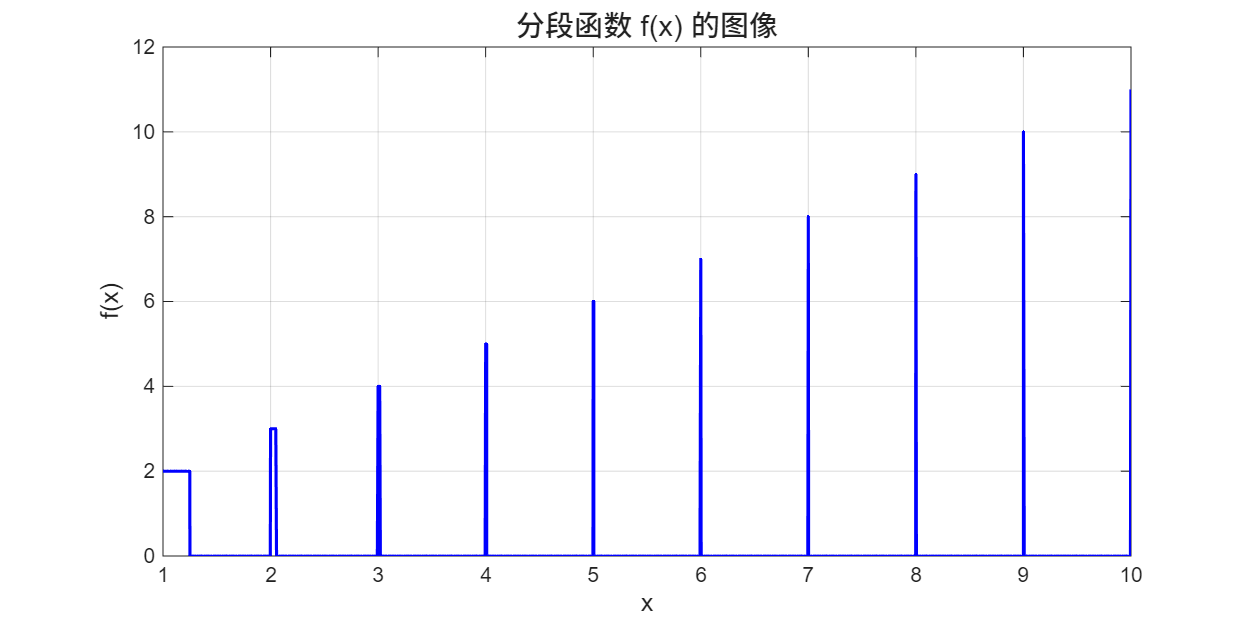
\includegraphics[width=0.7\linewidth]{figure/C7/untitled}
\end{center}

\begin{proof}
	对任意 $A>1$，取 $n \in \mathbb{N}$，使 $A \in [n,n+1)$.由 $f(x) \ge 0$，有
	\[
	\int_1^n f(x)\dd x \le \int_1^A f(x)\dd x \le \int_1^{n+1} f(x)\dd x
	\]
	
	当 $n \to +\infty$ 时，
	\[
	\begin{aligned}
		\lim_{n \to \infty} \int_1^n f(x)\dd x &= \lim_{n \to \infty} \left[ \int_1^2 f(x)\dd x + \dots + \int_{n-1}^n f(x)\dd x \right] \\
		&= \lim_{n \to \infty} \left[ \frac{1}{1 \cdot 2} + \frac{1}{2 \cdot 3} + \dots + \frac{1}{(n-1)n} \right] \\
		&= \lim_{n \to \infty} \left( 1 - \frac{1}{2} + \frac{1}{2} - \frac{1}{3} + \dots + \frac{1}{n-1} - \frac{1}{n} \right) \\
		&= \lim_{n \to \infty} \left( 1 - \frac{1}{n} \right) = 1
	\end{aligned}
	\]
	
	同理
	\[
	\lim_{n \to \infty} \int_1^{n+1} f(x)\dd x = 1
	\]
	由夹逼性
	\[
	\int_1^{+\infty} f(x)\dd x = 1
	\]
	
	
\end{proof} 
类似的方式，即使 $f(x)$ 在 $[a,+\infty)$ 连续（$n$ 次可微），也可以构造出使 $\displaystyle\int_a^{+\infty} f(x)dx$ 收敛而 $f(x)$ 在 $[a,+\infty)$ 无界的例子.

对反常积分的计算，我们可以形式上认为
\[
\int_a^{+\infty} f(x)\dd x = \lim_{A \to +\infty} F(A) - F(a)
\]

%
% 第7节：反常积分验敛法
% !TEX root = ../../../main.tex
% 所属：第一部分：单变量分析学 / 第8章：Riemann积分
% 节：8.7 反常积分验敛法
% 正文按原文件顺序保存；由 ../chapter8.tex 调用。
\section{反常积分验敛法}
\begin{proposition}（Cauchy 收敛原理）
	\[
	\int_a^{+\infty} f(x)\dd x \text{ 收敛} \iff
	\]
	$\forall \varepsilon>0$，$\exists M>0$ 且 $M \ge a$，使得 $\forall A_1,A_2 \ge M$，都有
	\[
	\left| \int_{A_2}^{A_1} f(x)\dd x \right| < \varepsilon
	\]
\end{proposition}
\begin{proof}
	由函数极限的 Cauchy 收敛原理易得.
\end{proof}
同时，我们给出无限区间上反常积分的 Cauchy 不收敛原理.

\begin{proposition}
	\[
	\int_a^{+\infty} f(x)\dd x \text{ 发散} \iff \exists \varepsilon_0>0,\ \forall M>0 \text{ 且 } M \ge a,\ \forall A_1,A_2 \ge M,
	\]
	都有
	\[
	\left| \int_{A_2}^{A_1} f(x)\dd x \right| \ge \varepsilon_0
	\]
	
\end{proposition}
\begin{definition}
	对 $f(x)$，若
	\[
	\int_a^{+\infty} |f(x)|\dd x
	\]
	收敛，则称 $\displaystyle\int_a^{+\infty} f(x)\dd x$ 绝对收敛，又称 $f(x)$ 在 $[a,+\infty)$ 绝对可积.
	
\end{definition}

\begin{proposition}
	若 $\displaystyle\int_a^{+\infty} f(x)\dd x$ 绝对收敛，则 $\displaystyle\int_a^{+\infty} f(x)\dd x$ 收敛.
\end{proposition}
\begin{proof}
	由 $\displaystyle\int_a^{+\infty} |f(x)|\dd x$ 收敛，$\forall \varepsilon>0$，$\exists M>0$ 且 $M \ge a$，使得 $\forall A_1,A_2 \ge M$ 且 $A_1>A_2$，有
	\[
	\int_{A_2}^{A_1} |f(x)|\dd x < \varepsilon
	\]
	而 $f \in \mathcal{R}[A_2,A_1]$，故
	\[
	\left| \int_{A_2}^{A_1} f(x)dx \right| \le \int_{A_2}^{A_1} |f(x)|\dd x < \varepsilon
	\]
	由Cauchy收敛原理，$\displaystyle\int_a^{+\infty} f(x)\dd x$ 收敛.
\end{proof}

\begin{definition}
	若 $\displaystyle\int_a^{+\infty} f(x)\dd x$ 收敛，但 $\displaystyle\int_a^{+\infty} |f(x)|\dd x$ 发散，则称 $\displaystyle\int_a^{+\infty} f(x)\dd x$ 条件收敛.
	
\end{definition}
下面我们考虑定号函数反常积分的敛散性
\begin{proposition}（比较验敛法）\label{比较验敛法}
	设函数 $f$ 在 $[a,+\infty)$ 上有定义，$\exists A \ge a$，使得 $f(x)$ 在 $[A,+\infty)$ 上满足 $f \ge 0$（或 $f \le 0$），函数 $\varphi$ 在 $[A,+\infty)$ 上满足
	\[
	0 \le f(x) \le k \varphi(x), \quad k \ge 0
	\]
	则
	\begin{enumerate}
		\item 若 $\displaystyle\int_a^{+\infty} \varphi(x)\dd x$ 收敛 $\implies \displaystyle\int_a^{+\infty} f(x)\dd x$ 收敛；
		\item 若 $\displaystyle\int_a^{+\infty} f(x)\dd x$ 发散 $\implies \displaystyle\int_a^{+\infty} \varphi(x)\dd x$ 发散.
	\end{enumerate}
	
	
\end{proposition}


\begin{proof}
	显然地，1 与 2 互为逆否命题，只需证明 1.
	
	由 $\displaystyle\int_a^{+\infty} \varphi(x)\dd x$ 收敛，根据 Cauchy 收敛准则，
	$\forall \varepsilon>0$，$\exists M \ge A$，$\forall A_1,A_2 \ge M$ 且 $A_1 \le A_2$，有
	\[
	0 < \int_{A_1}^{A_2} \varphi(x)\dd x < \varepsilon
	\]
	于是
	\[
	0 \le \int_{A_1}^{A_2} f(x)\dd x \le k \int_{A_1}^{A_2} \varphi(x)\dd x < k\varepsilon
	\]
	故 $\displaystyle\int_a^{+\infty} f(x)\dd x$ 收敛.
\end{proof} 
下面给出\ref{比较验敛法}的极限形式
\begin{corollary}
	设 $f(x)$ 与 $\varphi(x)$ 在 $[a,+\infty)$ 为非负函数，且
	\[
	\lim_{x \to +\infty} \frac{f(x)}{\varphi(x)} = l
	\]
	\begin{enumerate}
		\item 若 $0 \le l < +\infty$，则
		\[
		\int_a^{+\infty} \varphi(x)\dd x \text{ 收敛} \implies \int_a^{+\infty} f(x)\dd x \text{ 收敛}
		\] 
		\item  若 $0 < l \le +\infty$，则
		\[
		\int_a^{+\infty} \varphi(x)\dd x \text{ 发散} \implies \int_a^{+\infty} f(x)\dd x \text{ 发散}
		\]
	\end{enumerate}
	
	也就是说，$0<l<+\infty$时,$\varphi(x)$ 与 $f(x)$ 有相同的敛散性.
	
\end{corollary}
\begin{proof}
	\begin{enumerate}
		\item 由 $\lim\limits_{x \to +\infty} \dfrac{f(x)}{\varphi(x)} = l < +\infty$，则对 $\varepsilon=1$，$\exists M_0 \ge a$，当 $x > M_0$ 时
		\[
		0 \le \frac{f(x)}{\varphi(x)} - l < 1
		\]
		即
		\[
		0 \le l\varphi(x) \le f(x) \le (1+l)\varphi(x)
		\]
		由 $\displaystyle\int_a^{+\infty} \varphi(x)\dd x$ 收敛，推出 $\displaystyle\int_a^{+\infty} f(x)\dd x$ 收敛.
		
		\item 若 $0 < l \le +\infty$，令 $l' = \dfrac{1}{l}$，则 $0 \le l' < +\infty$，且
		\[
		\lim_{x \to +\infty} \frac{\varphi(x)}{f(x)} = l' \in [0,+\infty)
		\]
		对 $\varepsilon=1$，$\exists \widetilde{M}_0 \ge a$，$\forall x > \widetilde{M}_0$，有
		\[
		0 \le \frac{\varphi(x)}{f(x)} \le l' + 1
		\]
		即
		\[
		0 \le \varphi(x) \le (l'+1)f(x)
		\]
		由 $\displaystyle\int_a^{+\infty} \varphi(x)\dd x$ 发散，得 $\displaystyle\int_a^{+\infty} f(x)\dd x$ 发散.
	\end{enumerate}
\end{proof}
使用 $p$-积分与比较验敛法，我们得到 Cauchy 判别法.
\begin{corollary}
	（Cauchy 判别法）
	在 $[a,+\infty) \subset (0,+\infty)$ 上恒有 $f(x) \ge 0$，$K$ 是正常数.
	
	(1) 若 $f(x) \le \dfrac{K}{x^p}$，且 $p>1$，则 $\displaystyle\int_a^{+\infty} f(x)\dd x$ 收敛；
	
	(2) 若 $f(x) \ge \dfrac{K}{x^p}$，且 $p \le 1$，则 $\displaystyle\int_a^{+\infty} f(x)\dd x$ 发散.
\end{corollary}
\begin{corollary}
	（Cauchy 判别法的极限形式）
	设在 $[a,+\infty) \subset (0,+\infty)$ 上恒有 $f(x) \ge 0$，且
	\[
	\lim_{x \to +\infty} x^p f(x) = l
	\]
	则
	
	(1) 若 $0 \le l < +\infty$ 且 $p>1$，则 $\displaystyle\int_a^{+\infty} f(x)\dd x$ 收敛；
	
	(2) 若 $0 < l \le +\infty$ 且 $p \le 1$，则 $\displaystyle\int_a^{+\infty} f(x)\dd x$ 发散.
\end{corollary}


下面，我们先再次证明第二积分中值定理的一个特殊情况，证明的方法更有技巧性.
\begin{proposition}
	设 $f$ 在 $[a,b]$ 上连续且常义可积，$g$ 在 $[a,b]$ 上单调、连续可导且常义可积，则 $\exists \xi \in [a,b]$，使得
	\[
	\int_a^b f(x)g(x)\dd x = g(a)\int_a^\xi f(x)x + g(b)\int_\xi^b f(x)\dd x
	\]
\end{proposition}
\begin{proof}
	令 $F(x) = \displaystyle\int_a^x f(t)\dd t$，因 $f(x)$ 连续，故 $F'(x)=f(x)$.由分部积分法，
	\[
	\begin{aligned}
		\int_a^b f(x)g(x)\dd x &= \int_a^b g(x) d\left( \int_a^x f(t)\dd t \right) \\
		&= \left. g(x)F(x) \right|_a^b - \int_a^b F(x)g'(x)\dd x
	\end{aligned}
	\]
	因 $g$ 单调，故 $g'(x)$ 在 $[a,b]$ 上不变号，由积分第一中值定理，$\exists \xi \in [a,b]$，使得
	\[
	\int_a^b F(x)g'(x)dx = F(\xi)\int_a^b g'(x)\dd x
	\]
	代入上式得
	\[
	\begin{aligned}
		\int_a^b f(x)g(x)\dd x &= g(b)F(b) - F(\xi)\int_a^b g'(x)\dd x \\
		&= g(b)\int_a^b f(x)\dd x - \int_a^\xi f(x)\dd x \cdot \left( g(b)-g(a) \right) \\
		&= g(a)\int_a^\xi f(x)\dd x + g(b)\int_\xi^b f(x)\dd x
	\end{aligned}
	\]
\end{proof}

下面介绍 A-D 判别法.
\begin{proposition}(A-D 判别法)
	
	\begin{enumerate}
		\item Abel 判别法：若 $\displaystyle\int_a^{+\infty} f(x)\dd x$ 收敛，$g(x)$ 在 $[a,+\infty)$ 上单调有界，则 $\displaystyle\int_a^{+\infty} f(x)g(x)\dd x$ 收敛.
		\item Dirichlet 判别法：若 $F(A)=\displaystyle\int_a^A f(x)\dd x$ 在 $[a,+\infty)$ 上有界，$g(x)$ 在 $[a,+\infty)$ 上单调且 $\lim\limits_{x \to +\infty} g(x)=0$，则 $\displaystyle\int_a^{+\infty} f(x)g(x)\dd x$ 收敛.
	\end{enumerate}
\end{proposition}
\begin{proof}
	\begin{enumerate}
		\item 由 $g(x)$ 在 $[a,+\infty)$ 上有界，$\exists M \ge 0$，使得 $|g(x)| \le M$ 对 $\forall x \in [a,+\infty)$ 成立.
		因 $\displaystyle\int_a^{+\infty} f(x)\dd x$ 收敛，由 Cauchy 收敛准则，$\forall \varepsilon>0$，$\exists G \ge a$，对 $\forall A_1,A_2 > G$ 且 $A_1 < A_2$，有
		\[
		\left| \int_{A_1}^{A_2} f(x)\dd x \right| < \varepsilon
		\]
		由第二积分中值定理，$\exists \xi \in [A_1,A_2]$，使得
		\[
		\int_{A_1}^{A_2} f(x)g(x)dx = g(A_1)\int_{A_1}^\xi f(x)dx + g(A_2)\int_\xi^{A_2} f(x)dx
		\]
		因此
		\[
		\begin{aligned}
			\left| \int_{A_1}^{A_2} f(x)g(x)\dd x \right|
			&= \left| g(A_1)\int_{A_1}^\xi f(x)\dd x + g(A_2)\int_\xi^{A_2} f(x)\dd x \right| \\
			&\le |g(A_1)| \cdot \left| \int_{A_1}^\xi f(x)\dd x \right| + |g(A_2)| \cdot \left| \int_\xi^{A_2} f(x)\dd x \right| \\
			&\le M \left( \left| \int_{A_1}^\xi f(x)\dd x \right| + \left| \int_\xi^{A_2} f(x)\dd x \right| \right) \\
			&< 2M\varepsilon
		\end{aligned}
		\]
		由 Cauchy 收敛准则，$\displaystyle\int_a^{+\infty} f(x)g(x)\dd x$ 收敛.
		\item 由 $F(A)=\displaystyle\int_a^A f(x)\dd x$ 在 $[a,+\infty)$ 上有界，$\exists L>0$，对 $\forall A \in [a,+\infty)$，有
		\[
		|F(A)| = \left| \int_a^A f(x)\dd x \right| < L
		\]
		由 $\lim\limits_{x \to +\infty} g(x)=0$，$\forall \varepsilon>0$，$\exists X > a$，对 $\forall x > X$，有 $|g(x)| < \varepsilon$.
		对 $\forall A_1,A_2 > X$ 且 $A_1 \le A_2$，有 $|g(A_1)| < \varepsilon$，$|g(A_2)| < \varepsilon$.
		由第二积分中值定理，$\exists \xi \in [A_1,A_2]$，使得
		\[
		\int_{A_1}^{A_2} f(x)g(x)\dd x = g(A_1)\int_{A_1}^\xi f(x)\dd x + g(A_2)\int_\xi^{A_2} f(x)\dd x
		\]
		因此
		\[
		\begin{aligned}
			\left| \int_{A_1}^{A_2} f(x)g(x)\dd x \right|
			&= \left| g(A_1)\int_{A_1}^\xi f(x)\dd x + g(A_2)\int_\xi^{A_2} f(x)\dd x \right| \\
			&\le |g(A_1)| \cdot \left| \int_{A_1}^\xi f(x)\dd x \right| + |g(A_2)| \cdot \left| \int_\xi^{A_2} f(x)\dd x \right| \\
			&< \varepsilon \left( \left| \int_a^\xi f(x)\dd x - \int_a^{A_1} f(x)\dd x \right| + \left| \int_a^{A_2} f(x)\dd x - \int_a^\xi f(x)\dd x \right| \right) \\
			&< \varepsilon (L + L + L + L) = 4L\varepsilon
		\end{aligned}
		\]
		由 Cauchy 收敛准则，$\displaystyle\int_a^{+\infty} f(x)g(x)\dd x$ 收敛.
	\end{enumerate}
	
	
\end{proof}
\begin{example}
	考虑反常积分 $$ \int_0^{+\infty} \frac{\sin x}{x} \dd x$$ 的敛散性.
\end{example}
\begin{solution}
	将积分拆分为两部分：
	\[
	\int_0^{+\infty} \frac{\sin x}{x} dx = \int_0^1 \frac{\sin x}{x} dx + \int_1^{+\infty} \frac{\sin x}{x} dx = I + J
	\]
	
	对于 $I = \displaystyle\int_0^1 \dfrac{\sin x}{x} \dd x$：
	由于 $\lim\limits_{x\to0} \dfrac{\sin x}{x} = 1$，因此被积函数在 $x=0$ 附近有界，$I$ 是常义（Riemann）积分，必然收敛.
	
	对于 $J = \displaystyle\int_1^{+\infty} \dfrac{\sin x}{x} \dd x$：
	应用 Dirichlet 判别法：
	令 $f(x) = \sin x$，$g(x) = \dfrac{1}{x}$.
	
	1.  $F(A) = \displaystyle\int_1^A \sin x \dd x = -\cos A + \cos 1$ 在 $[1,+\infty)$ 上显然有界.
	
	2.  $g(x) = \dfrac{1}{x}$ 在 $[1,+\infty)$ 上单调递减，且 $\lim\limits_{x\to+\infty} g(x) = 0$.
	故 $J$ 收敛，因此原积分 $\displaystyle \int_0^{+\infty} \dfrac{\sin x}{x} \dd x$ 收敛.
	
	接下来判断其是否绝对收敛：
	\[
	\int_0^{+\infty} \left| \frac{\sin x}{x} \right| \dd x \ge \int_0^{+\infty} \frac{|\sin x|}{x} \dd x
	\]
	利用恒等式 $|\sin x|^2 = \sin^2 x = \dfrac{1-\cos 2x}{2}$，有：
	\[
	\int_0^{+\infty} \frac{|\sin x|}{x} \dd x \ge \int_0^{+\infty} \frac{\sin^2 x}{x} \dd x = \int_0^{+\infty} \frac{1-\cos 2x}{2x} \dd x = \int_0^{+\infty} \frac{1}{2x} \dd x - \int_0^{+\infty} \frac{\cos 2x}{2x} \dd x
	\]
	其中，$\displaystyle \int_0^{+\infty} \frac{1}{2x} dx$ 是 $p=1$ 的 $p$-积分，发散因此，原不等式右边整体发散，从而 $\displaystyle \int_0^{+\infty} \left| \frac{\sin x}{x} \right| dx$ 发散.
	
	综上，$\displaystyle \int_0^{+\infty} \frac{\sin x}{x} \dd x$ 条件收敛.
\end{solution}
对于有限闭区间上的无界函数的反常积分
\[
\int_a^b f(x)\dd x
\]
且 \(f(x)\) 在 \([a,b]\) 上有唯一的奇点 \(b\)。我们作变换
\[
t=\frac{1}{b-x},
\]
那么
\[
I=\int_a^b f(x)\dd x=\int_{\tfrac{1}{b-a}}^{+\infty} \frac{1}{t^2} f\left(b-\frac{1}{t}\right) \dd t.
\]
我们可以得到对应的 Cauchy 收敛原理、Cauchy 判别法与 A-D 判别法。
\begin{proposition}
	对上述的 $\displaystyle \int_a^b f(x)\dd x$ 收敛的充分必要条件是：
	$\forall \varepsilon>0,\ \exists \delta>0$，对任意 $\eta,\eta' \in (0,\delta)$，有
	\[
	\left| \int_{b-\eta}^{b-\eta'} f(x)\dd x \right| < \varepsilon
	\]
\end{proposition}
\begin{proposition}
	设在 $[a,b)$ 上恒有 $f(x) \ge 0$，若当 $x$ 属于 $b$ 的某个左邻域 $[b-\eta_0,b)$ 时，存在正常数 $K$与函数$\varphi(x)$，使得
	\begin{enumerate}
		\item 若 $f(x) \le K\varphi(x)$ 且 $\displaystyle\int_a^b \varphi(x)\dd x$收敛，则 $\displaystyle \int_a^b f(x)\dd x$ 收敛；
		\item 若 $f(x) \ge  K\varphi(x)$ 且$\displaystyle\int_a^b \varphi(x)\dd x$发散，则 $\displaystyle \int_a^b f(x)\dd x$ 发散。
	\end{enumerate}
\end{proposition}
\begin{proposition}
	设在 $[a,b)$ 上恒有 $f(x),\varphi(x) \ge 0$，且
	\[
	\lim_{x \to b^-} \dfrac{f(x)}{\varphi(x)} = l
	\]
	则
	\begin{enumerate}
		\item 若 $0 \le l < +\infty$ 且 $\displaystyle\int_a^b \varphi(x)\dd x$收敛，则 $\displaystyle \int_a^b f(x)\dd x$ 收敛；
		\item 若 $0 < l \le +\infty$ 且 $\displaystyle\int_a^b \varphi(x)\dd x$发散，则 $\displaystyle \int_a^b f(x)\dd x$ 发散。
	\end{enumerate}
	
\end{proposition}
\begin{proposition}
	设在 $[a,b)$ 上恒有 $f(x) \ge 0$，若当 $x$ 属于 $b$ 的某个左邻域 $[b-\eta_0,b)$ 时，存在正常数 $K$，使得\begin{enumerate}
		\item 若 $f(x) \le \dfrac{K}{(b-x)^p}$ 且 $p<1$，则 $\displaystyle \int_a^b f(x)\dd x$ 收敛；
		\item 若 $f(x) \ge \dfrac{K}{(b-x)^p}$ 且 $p \ge 1$，则 $\displaystyle \int_a^b f(x)\dd x$ 发散。
	\end{enumerate}
\end{proposition}
\begin{proposition}
	设在 $[a,b)$ 上恒有 $f(x) \ge 0$，且
	\[
	\lim_{x \to b^-} (b-x)^p f(x) = l
	\]
	则
	\begin{enumerate}
		\item 若 $0 \le l < +\infty$ 且 $p<1$，则 $\displaystyle \int_a^b f(x)\dd x$ 收敛；
		\item 若 $0 < l \le +\infty$ 且 $p \ge 1$，则 $\displaystyle \int_a^b f(x)\dd x$ 发散。
	\end{enumerate}
	
\end{proposition}
\begin{proposition}
	若下列两个条件之一满足，则 $\displaystyle \int_a^b f(x)g(x)\dd x$ 收敛：
	\begin{enumerate}
		\item \textbf{Abel 判别法}：$\displaystyle \int_a^b f(x)\dd x$ 收敛，$g(x)$ 在 $[a,b)$ 上单调有界；
		\item \textbf{Dirichlet 判别法}：$F(\eta)=\displaystyle \int_a^{b-\eta} f(x)\dd x$ 在 $(0,b-a]$ 上有界，$g(x)$ 在 $[a,b)$ 上单调且 $\lim_{x \to b^-} g(x)=0$。
	\end{enumerate}
\end{proposition}
\begin{proposition}
	设 $f(x)$ 在 $[a,+\infty)$ 上一致连续，且反常积分 $\displaystyle \int_a^{+\infty} f(x)\dd x$ 收敛，则
	\[
	\lim_{x\to+\infty} f(x)=0\]
\end{proposition}
\begin{proof}
	（反证法）
	若不然，即 $\lim\limits_{x\to+\infty} f(x)\neq 0$，则 $\exists \varepsilon_0>0$，对任意 $M>0$，总能找到 $x_0>M$，使得 $|f(x_0)|\ge \varepsilon_0$。
	
	取 $M_1=a+1$，则 $\exists x_1>M_1$，但 $|f(x_1)|\ge \varepsilon_0$；
	
	再取 $M_2=x_1+1$，则 $\exists x_2>M_2$，但$|f(x_2)|\ge \varepsilon_0$；
	
	$\vdots$
	
	以此类推，我们可以得到一个严格单调递增趋于 $+\infty$ 的数列 $\{x_n\}_{n=1}^\infty \subset [a,+\infty)$，满足 $|f(x_n)|\ge \varepsilon_0$。
	
	由于数列有无穷多个点，$f(x_n)$ 要么恒正，要么恒负。不失一般性，我们假设所有 $f(x_n)\ge \varepsilon_0>0$。
	
	由 $f(x)$ 在 $[a,+\infty)$ 上一致连续，对 $\dfrac{\varepsilon_0}{2}>0$，$\exists \delta_0>0$，使得对任意 $x',x''$，只要 $0<|x'-x''|<\delta_0$，就有
	\[
	|f(x')-f(x'')|<\frac{\varepsilon_0}{2}
	\]
	特别地，对任意 $x$ 满足 $|x-x_n|<\delta_0$，有
	\[
	f(x) > f(x_n) - \frac{\varepsilon_0}{2} \ge \varepsilon_0 - \frac{\varepsilon_0}{2} = \frac{\varepsilon_0}{2}
	\]
	因此，对任意 $n\ge 1$，有
	\[
	\int_{x_n-\delta_0/2}^{x_n+\delta_0/2} f(x)dx \ge \int_{x_n-\delta_0/2}^{x_n+\delta_0/2} \frac{\varepsilon_0}{2} dx = \delta_0 \cdot \frac{\varepsilon_0}{2} = C_0
	\]
	其中 $C_0=\dfrac{\delta_0\varepsilon_0}{2}>0$ 是一个常数。
	
	令 $y_n=x_n+\delta_0/2$，$y'_n=x_n-\delta_0/2$，则得到两个数列 $\{y_n\}$ 和 $\{y'_n\}$，它们都严格单调趋于 $+\infty$，且满足
	\[
	\int_{y'_n}^{y_n} f(x)dx \ge C_0
	\]
	这与反常积分 $\displaystyle \int_a^{+\infty} f(x)\dd x$ 收敛的 Cauchy 准则矛盾。
	
	因此，原命题成立，即 $\displaystyle \lim_{x\to+\infty} f(x)=0$。
	
	
\end{proof}
%
% 第8节：积分与级数
% !TEX root = ../../../main.tex
% 所属：第一部分：单变量分析学 / 第8章：Riemann积分
% 节：8.8 积分与级数
% 正文按原文件顺序保存；由 ../chapter8.tex 调用。
\section{积分与级数}
\begin{proposition}（积分判别法）
	设函数 $f(x)$ 在 $[a, +\infty)$ 上恒大于等于 $0$，取一个严格单调上升且趋于 $+\infty$ 的数列 $a_1 = a < a_2 < a_3 < \dots$，令
	\[
	u_n = \int_{a_n}^{a_{n+1}} f(x) \dd x
	\]
	则级数 $\sum u_n$ 与反常积分 $\displaystyle\int_{a}^{+\infty} f(x) \dd x$ 有相同的敛散性，并且当它们收敛时，
	\[
	\sum_{n=1}^{\infty} u_n = \int_{a}^{+\infty} f(x) \dd x
	\]
\end{proposition}



注意：当 $f(x) \ge 0$ 不成立时，由 $\displaystyle\int_{a}^{+\infty} f(x) \dd x$ 收敛可推得 $\sum u_n$ 收敛，但反之不成立。
例如：反常积分 $\displaystyle\int_{a}^{+\infty} \sin x \dd x$ 发散，但取 $u_n = \displaystyle\int_{n\pi}^{2n\pi} \sin x \dd x = 0$，此时级数 $\sum u_n$ 收敛。
\begin{proof}
	令 $F(A) = \displaystyle\int_{a}^{A} f(x) \dd x$。对任意 $A \ge a$，存在 $n$ 使得 $a_n \le A \le a_{n+1}$。设 $\sum u_n$ 的部分和为 $S_n$，则
	\begin{align*}
		\int_{a}^{A} f(x) \dd x
		&= \sum_{i=1}^{n-1} \int_{a_i}^{a_{i+1}} f(x) \dd x + \int_{a_n}^{A} f(x) \dd x \\
		&= S_{n-1} + \int_{a_n}^{A} f(x) \dd x
	\end{align*}
	由于 $f(x) \ge 0$，有
	\[
	S_{n-1} \le \int_{a}^{A} f(x) \dd x \le S_{n-1} + \int_{a_n}^{a_{n+1}} f(x) \dd x = S_n
	\]
	即
	\[
	S_{n-1} \le F(A) \le S_n
	\]
	\begin{itemize}
		\item 若 $\sum u_n$ 发散，则 $\{S_n\}$ 发散，从而 $F(A) \to +\infty$，即反常积分发散。
		\item 若 $\sum u_n$ 收敛，则 $\{S_n\}$ 收敛，从而 $F(A)$ 收敛，即反常积分收敛。
	\end{itemize}
	
	
	
\end{proof}
特别地，当 $f(x)$ 单调减少时，取 $a_n = n$，则当 $n \ge N = \lfloor a \rfloor + 1$ 时，有
\[
f(n+1) \le u_n = \int_{n}^{n+1} f(x) \dd x \le f(n)
\]
由比较判别法可知，级数 $\sum_{n=1}^{\infty} f(n)$ 与 $\sum_{n=1}^{\infty} u_n$ 同时收敛或发散，从而 $\sum_{n=1}^{\infty} f(n)$ 与反常积分 $\displaystyle\int_{a}^{+\infty} f(x) \dd x$ 同时收敛或发散。
\begin{example}
		考虑级数 $\sum_{n=2}^{\infty} \dfrac{1}{n(\ln n)^p}$ 的敛散性。
\end{example}


\begin{proof}
	与 \ref{级数1/nlnn}不同，我们用积分判别法来做。
	由积分判别法，级数 $\sum\limits_{n=2}^{\infty} \dfrac{1}{n(\ln n)^p}$ 与反常积分 $\displaystyle\int_{2}^{+\infty} \frac{1}{x(\ln x)^p} \mathrm{d}x$ 有相同的敛散性。
	
	故只需考虑反常积分 $\displaystyle\int_{2}^{+\infty} \frac{1}{x(\ln x)^p} \dd x$ 的敛散性。
	
	\[
	\int_{2}^{+\infty} \frac{1}{x(\ln x)^p} \dd x
	= \int_{2}^{+\infty} \frac{1}{(\ln x)^p} \dd (\ln x)
	=
	\begin{cases}
		\ln \ln x \Big|_{2}^{+\infty} \to +\infty, & p=1 \\[6pt]
		\dfrac{1}{1-p} (\ln x)^{1-p} \Big|_{2}^{+\infty}, & p \ne 1
	\end{cases}
	\]
	
	当 $1-p < 0$，即 $p>1$ 时，反常积分收敛；当 $p \le 1$ 时，反常积分发散。
	
	因此，级数 $\sum\limits_{n=2}^{\infty} \dfrac{1}{n(\ln n)^p}$ 当 $p>1$ 时收敛，当 $p \le 1$ 时发散。
	
\end{proof}
\begin{example}
	证明：
	
	1.  $\displaystyle \int_{0}^{+\infty} \frac{\dd x}{1+x^2\sin^2 x}$ 发散
	
	2.  $\displaystyle \int_{0}^{+\infty} \frac{\dd x}{1+x^4\sin^2 x}$ 收敛
\end{example}
\begin{solution}
	(1) 取 $a_n = n\pi,\ n=0,1,2,\dots$，令
	\[
	u_n = \int_{n\pi}^{(n+1)\pi} \frac{\dd x}{1+x^2\sin^2 x}
	= \int_{0}^{\pi} \frac{\dd t}{1+(n\pi+t)^2\sin^2 t}
	> \int_{0}^{\frac{1}{(n+1)\pi}} \frac{\dd t}{1+(n\pi+t)^2\sin^2 t}
	\]
	当 $0 < t < \dfrac{1}{(n+1)\pi}$ 时，有
	\[
	(n\pi+t)^2\sin^2 t < (n+1)^2\pi^2 t^2 < (n+1)^2\pi^2 \cdot \frac{1}{(n+1)^2\pi^2} = 1
	\]
	于是
	\[
	u_n > \int_{0}^{\frac{1}{(n+1)\pi}} \frac{\dd t}{1+1} = \frac{1}{2} \cdot \frac{1}{(n+1)\pi} = \frac{1}{2\pi} \cdot \frac{1}{n+1}
	\]
	因为级数 $\sum \dfrac{1}{n+1}$ 发散，由比较判别法可知 $\sum u_n$ 发散，故由积分判别法得 $\displaystyle \int_{0}^{+\infty} \frac{\dd x}{1+x^2\sin^2 x}$ 发散。
	
	(2) 取 $a_n = n\pi,\ n=0,1,2,\dots$，令
	\[
	u_n = \int_{n\pi}^{(n+1)\pi} \frac{\dd x}{1+x^4\sin^2 x}
	= \int_{0}^{\pi} \frac{\dd t}{1+(n\pi+t)^4\sin^2 t}
	\]
	将积分拆为两部分：
	\[
	u_n = \int_{0}^{\frac{\pi}{2}} \frac{\dd t}{1+(n\pi+t)^4\sin^2 t} + \int_{0}^{\frac{\pi}{2}} \frac{\dd t}{1+(n\pi+\pi-t)^4\sin^2 t} = u_n' + u_n''
	\]
	当 $0 < t < \dfrac{\pi}{2}$ 时，有 $\sin t \ge \dfrac{2}{\pi}t$，故
	\[
	(n\pi+t)^4\sin^2 t \ge n^4\pi^4 \left(\frac{2t}{\pi}\right)^2 = 4\pi^2n^4t^2
	\]
	于是
	\[
	u_n' \le \int_{0}^{\frac{\pi}{2}} \frac{\dd t}{1+4\pi^2n^4t^2}
	= \frac{1}{2\pi n^2} \int_{0}^{\pi^2n^2} \frac{\dd s}{1+s^2}
	< \frac{1}{2\pi n^2} \cdot \frac{\pi}{2} = \frac{1}{4n^2}
	\]
	由于级数 $\sum \dfrac{1}{n^2}$ 收敛，故 $\sum u_n'$ 收敛；同理可证 $\sum u_n''$ 收敛，因此 $\sum u_n$ 收敛，故由积分判别法得 $\displaystyle \int_{0}^{+\infty} \frac{\dd x}{1+x^4\sin^2 x}$ 收敛。
\end{solution}












































%
